\documentclass[12pt,a4paper,oneside]{report}

% ─── Packages ──────────────────────────────────────────────────────────────────
\usepackage[margin=2.5cm, top=3cm, bottom=3cm, headheight=14.5pt]{geometry}
\usepackage[T1]{fontenc}
\usepackage[utf8]{inputenc}
\usepackage{lmodern}
\usepackage{graphicx}
\usepackage{booktabs}
\usepackage{longtable}
\usepackage{array}
\usepackage{tabularx}
\usepackage{xcolor}
\usepackage{enumitem}
\usepackage{parskip}
\usepackage{titlesec}
\usepackage[hidelinks]{hyperref}
\usepackage{mdframed}
\usepackage{subcaption}
\usepackage{float}
\usepackage{fancyhdr}
\usepackage{emptypage}
\usepackage{tocloft}
\usepackage{amsmath}
\usepackage{pdflscape}

% ─── Colors ────────────────────────────────────────────────────────────────────
\definecolor{gold}{HTML}{D4AF37}
\definecolor{darkbg}{HTML}{0A0E14}
\definecolor{midgray}{HTML}{555555}

% ─── Chapter / section formatting ──────────────────────────────────────────────
\titleformat{\chapter}[display]
  {\normalfont\huge\bfseries}{\chaptertitlename\ \thechapter}{16pt}{\Huge}
\titlespacing*{\chapter}{0pt}{-10pt}{20pt}

\titleformat{\section}{\large\bfseries}{\thesection}{1em}{}[\titlerule]
\titleformat{\subsection}{\normalsize\bfseries}{\thesubsection}{1em}{}
\titleformat{\subsubsection}{\normalsize\bfseries\itshape}{\thesubsubsection}{1em}{}

% ─── Header / footer ───────────────────────────────────────────────────────────
\pagestyle{fancy}
\fancyhf{}
\fancyhead[L]{\small\textit{Spotly --- ISS296 --- Spring 2026}}
\fancyhead[R]{\small\textit{\leftmark}}
\fancyfoot[C]{\thepage}
\renewcommand{\headrulewidth}{0.4pt}

% ─── Graphics path ─────────────────────────────────────────────────────────────
% Searches both the same directory (nav.png, class.png) and the wireframe folder
\graphicspath{{./}{../../e2e/wireframes/screenshots/}{../../e2e/wireframes/sketches/}}

% ─── Misc helpers ──────────────────────────────────────────────────────────────
\newcolumntype{L}[1]{>{\raggedright\arraybackslash}p{#1}}
\setlength{\parskip}{6pt}

\hypersetup{
  colorlinks  = true,
  linkcolor   = black,
  urlcolor    = black,
  pdfauthor   = {Cyrine Krichen, Eya Sassi, Lina Khemiri, Youssef Ben Jemaa},
  pdftitle    = {Spotly --- ISS296 Project Report --- Spring 2026},
}

% ─── Scenario box (Appendix) ───────────────────────────────────────────────────
\mdfdefinestyle{scenariobox}{
  linecolor=black!25, linewidth=0.6pt,
  topline=true, bottomline=true, leftline=true, rightline=true,
  innertopmargin=6pt, innerbottommargin=6pt,
  innerleftmargin=8pt, innerrightmargin=8pt,
  skipabove=8pt, skipbelow=4pt
}

% ═══════════════════════════════════════════════════════════════════════════════
\begin{document}
\sloppy
% ═══════════════════════════════════════════════════════════════════════════════

% ─── Cover Page ────────────────────────────────────────────────────────────────
\begin{titlepage}
\pagestyle{empty}
\begin{center}


\includegraphics[height=2.2cm]{../../../LogoMedTech.png}

\vspace{1.2cm}

{\fontsize{11}{13}\selectfont\scshape
  Mediterranean Institute of Technology --- MedTech\\[0.3em]
  ISS296 --- Sophomore Project\\[0.3em]
  Spring 2026}

\vspace{2.5cm}

\rule{\linewidth}{0.6pt}\\[0.5em]
{\fontsize{32}{38}\selectfont\bfseries Spotly}\\[0.4em]
{\Large Luxury Venue Discovery and Booking Platform}\\[0.4em]
\rule{\linewidth}{0.6pt}

\vspace{2cm}

\begin{tabular}{rl}
  \textbf{Instructor:}  & Mr.\ Amine Ben Hassouna \\
                        & \href{mailto:amine.benhassouna@medtech.tn}%
                               {\texttt{amine.benhassouna@medtech.tn}} \\[1em]
  \textbf{Team:}        & Cyrine Krichen \\
                        & Eya Sassi \\
                        & Lina Khemiri \\
                        & Youssef Ben Jemaa \\
\end{tabular}

\vspace{2.5cm}

{\large Spring Semester 2026}

\vfill

{\small Academic Year 2025--2026}

\end{center}
\end{titlepage}

% ─── Front matter ──────────────────────────────────────────────────────────────
\pagenumbering{roman}
\setcounter{page}{1}

% ── Acknowledgement ────────────────────────────────────────────────────────────
\chapter*{Acknowledgement}
\addcontentsline{toc}{chapter}{Acknowledgement}
\markboth{Acknowledgement}{}

We would like to express our sincere gratitude to our supervisor,
\textbf{Mr.\ Amine Ben Hassouna}, for his guidance, availability, and
constructive feedback throughout the semester. His support was instrumental in
shaping both the scope and the quality of this project.

We also thank the \textbf{Mediterranean Institute of Technology} for providing
the academic framework and resources that made this project possible.

Finally, we thank each other. This project demanded genuine collaboration ---
across long evenings of learning, debugging, and polishing --- and we are proud
of what we built together.

\vspace{2em}
\noindent\textit{Cyrine Krichen, Eya Sassi, Lina Khemiri, Youssef Ben Jemaa}

% ── Table of Contents ──────────────────────────────────────────────────────────
\clearpage
\tableofcontents

% ── List of Figures ────────────────────────────────────────────────────────────
\listoffigures

\clearpage
\pagenumbering{arabic}
\setcounter{page}{1}

% ─── Introduction ──────────────────────────────────────────────────────────────
\chapter*{Introduction}
\addcontentsline{toc}{chapter}{Introduction}
\markboth{Introduction}{}

This report documents the design, planning, and implementation of
\textbf{Spotly}, the project produced by our team for the ISS296 course
during the Spring 2026 semester at the Mediterranean Institute of Technology.

\textbf{ISS296} is an integrated project course that challenges students to
conceive, design, and deliver a complete software application over a full
semester. The course covers the full development cycle: from requirements
elicitation and UML modelling, through UI design and iterative implementation,
to final documentation and presentation. The goal is to apply, in a realistic
setting, the techniques learned across the preceding semesters.

The domain we chose is \textbf{luxury venue discovery and table booking}. The
hospitality sector --- upscale restaurants, rooftop bars, private dining clubs,
lounges --- represents a context where the user experience has historically
lagged behind other consumer verticals. Reservations are still mostly handled
by phone or through generic booking platforms that offer no sense of the
venue's identity. We wanted to build something that felt as premium as the
venues it lists: a platform where discovery, booking, and floor management are
all tightly integrated and visually refined.

Spotly is a single-page application built entirely on the frontend. There is no
backend server; all data is persisted in the browser's \texttt{localStorage},
enabling cross-tab reactivity through the browser's native \texttt{storage}
event. This constraint was set by the course and pushed us to make thoughtful
choices about state management and data architecture.

After completing the core platform, the team went further by introducing a suite
of AI-powered features using the Groq inference API. These additions --- semantic
venue discovery, reservation insights, and a voice reservation agent --- were not
planned at the outset. They emerged from a shared desire to explore what the
platform could become, and they turned out to be the most technically challenging
and rewarding part of the project.

The report is structured as follows: Chapter~1 covers the analysis and
requirement specification; Chapter~2 describes the project planning;
Chapter~3 presents the software design artefacts; Chapter~4 details the
implementation; and the General Conclusion reflects on what we achieved and
what we would do next. The Appendix contains the full set of use case scenarios.


% ═══════════════════════════════════════════════════════════════════════════════
\chapter{Analysis and Requirement Specification}
\chaptermark{Analysis \& Requirements}
% ═══════════════════════════════════════════════════════════════════════════════

\section{Introduction}

This chapter establishes the foundation of the Spotly project. We define what
the platform is, what it aims to achieve, who it serves, and what value it
delivers. We then enumerate the system roles and the full feature set across
both phases of development.

\section{Description of the Project}

Spotly is a luxury venue discovery and table booking platform. It allows clients
to explore a curated list of high-end venues, inspect their profiles, and
complete a full booking flow ending with a reservation request that the venue
administrator reviews and processes.

On the operations side, Spotly provides venue administrators with a complete
management suite: floor plan builder, menu management, reservation queue,
review moderation, QR code generation, and venue identity settings. A separate
staff interface allows on-shift employees to manage the live floor in real time.

The platform is implemented as a frontend-only single-page application using
Vue.js~3 and Vuetify~3, with \texttt{localStorage} as the persistence layer.
The design language is built around a champagne gold (\texttt{\#D4AF37}) and
midnight black (\texttt{\#0A0E14}) palette, targeting a premium aesthetic.

\section{Objectives}

The primary objectives of the Spotly project are:

\begin{enumerate}[leftmargin=2em, topsep=4pt, itemsep=3pt]
  \item Deliver a complete, polished client-facing experience: venue discovery,
        filtering, profile browsing, and a multi-step booking flow.
  \item Deliver a comprehensive admin suite covering all aspects of venue
        configuration and daily operations.
  \item Deliver a staff operations dashboard for real-time floor management
        during service hours.
  \item Explore AI integration as a natural extension of the platform, adding
        value through semantic search, operational insights, and a conversational
        voice booking agent.
  \item Apply and demonstrate the full web development stack learned during the
        course: HTML5, CSS3, JavaScript, Vue.js, and Vuetify.
  \item Maintain a clean, documented, and maintainable codebase following the
        data-layer architecture required by the course.
\end{enumerate}

\section{Target Customers}

Spotly addresses three distinct customer segments:

\begin{itemize}[leftmargin=2em, topsep=4pt, itemsep=3pt]
  \item \textbf{Venue Clients.} Young professionals and experience-seekers aged
        22--45 who value aesthetics and convenience. They want to discover venues
        matching their mood, book a table without a phone call, and track their
        reservation in real time.

  \item \textbf{Venue Owners and Administrators.} Owners or managers of
        upscale restaurants, bars, and private dining spaces who need a
        streamlined system to manage reservations, configure their floor layout,
        maintain their digital menu, and monitor guest reviews.

  \item \textbf{Venue Staff.} On-shift waiters and hosts who need a simple,
        real-time tool to check in guests, handle walk-ins, and respond to
        table calls during service --- without the overhead of a full management
        interface.
\end{itemize}

\section{Value Proposition}

\begin{tabularx}{\linewidth}{>{\bfseries}lX}
  \toprule
  For & Value delivered \\
  \midrule
  Clients &
    A single destination to discover, explore, and book luxury venues ---
    with real-time status updates, AI-powered search, and a first-of-its-kind
    voice booking experience that requires no form filling. \\
  \addlinespace
  Admins &
    A self-contained operations hub: configure environments and tables
    visually, manage menus, process bookings, moderate reviews, generate QR
    codes, and read AI-generated insights --- all from one dashboard. \\
  \addlinespace
  Staff &
    A live floor map showing every table's state at a glance, with one-tap
    actions for check-in, no-show, walk-in, and waiter call acknowledgement. \\
  \bottomrule
\end{tabularx}

\section{System Roles}

Spotly distinguishes four user roles. A user's role is derived at runtime
from their account's relationship to venue data --- no role field is stored on
the \texttt{User} record.

\begin{tabularx}{\linewidth}{>{\bfseries}lX}
  \toprule
  Role & Description \\
  \midrule
  Guest &
    An unauthenticated visitor. Guests can browse the landing page, explore
    venues, view venue profiles, and scan QR codes to read the digital menu.
    They cannot make reservations or access any dashboard. \\
  \addlinespace
  Client &
    An authenticated user who is neither a venue owner nor assigned as staff.
    Clients can complete the full booking flow, track reservation status in
    real time, manage their bookings from the client dashboard, and submit
    reviews after a completed visit. \\
  \addlinespace
  Admin &
    A user whose email matches the \texttt{adminEmail} field of a
    \texttt{Venue} record. Admins have full control over their venue:
    floor plan, menu, reservations queue, reviews, QR codes, and identity
    settings. A user becomes an admin by completing venue onboarding after
    registration. \\
  \addlinespace
  Staff &
    A user linked to a venue through a \texttt{VenueStaff} record assigned
    by the admin. Staff operate the live floor: guest check-in, no-show
    marking, walk-in creation, and waiter call acknowledgement. \\
  \bottomrule
\end{tabularx}

\section{Features}

\subsection{Phase 1 --- Core Features}

\textbf{F1 --- User Authentication.}
Covers the full identity lifecycle of a user in the system.
\begin{itemize}[leftmargin=1.5em, topsep=2pt, itemsep=1pt]
  \item Register a new account with first name, last name, email, and password.
  \item Log in with existing credentials; session is persisted in
        \texttt{localStorage} under the key \texttt{spotly\_session}.
  \item Log out and invalidate the current session.
\end{itemize}

\textbf{F2 --- Venue Discovery and Search.}
Enables users to find venues matching their interests.
\begin{itemize}[leftmargin=1.5em, topsep=2pt, itemsep=1pt]
  \item Browse the full list of available venues on the home page.
  \item Search venues by name using a live search bar.
  \item Filter venues by activity type using toggle pill chips.
\end{itemize}

\textbf{F3 --- Venue Public Profile.}
Presents a venue's complete identity to any visitor.
\begin{itemize}[leftmargin=1.5em, topsep=2pt, itemsep=1pt]
  \item View venue name, description, tagline, location, ambience tags,
        activities, dress code, and supported languages.
  \item Browse the venue photo slideshow (hosted on Cloudinary).
  \item Read published guest reviews and overall rating.
\end{itemize}

\textbf{F4 --- Digital Menu.}
Provides a QR-accessible menu scoped to the guest's table environment.
\begin{itemize}[leftmargin=1.5em, topsep=2pt, itemsep=1pt]
  \item Browse menu items organised by category (starters, mains, desserts,
        drinks).
  \item View item name, description, price, allergens, and tags.
  \item Display only items available in the scanned table's environment when
        \texttt{environmentIds} scoping is configured on the menu item.
\end{itemize}

\textbf{F5 --- Booking: Environment Selection.}
First step of the booking flow.
\begin{itemize}[leftmargin=1.5em, topsep=2pt, itemsep=1pt]
  \item View all environments configured for the selected venue.
  \item Select an environment to continue to seat selection.
\end{itemize}

\textbf{F6 --- Booking: Seat and Table Selection.}
Second step of the booking flow.
\begin{itemize}[leftmargin=1.5em, topsep=2pt, itemsep=1pt]
  \item View the visual floor plan of the selected environment with live
        table availability derived from existing reservations.
  \item Select an available table and choose a reservation date and time.
\end{itemize}

\textbf{F7 --- Reservation Submission.}
Third step of the booking flow.
\begin{itemize}[leftmargin=1.5em, topsep=2pt, itemsep=1pt]
  \item Fill in reservation details: name, email, phone, number of guests,
        and optional notes.
  \item Submit the reservation request; status is set to \texttt{REQUESTED}.
  \item A double-submit guard prevents accidental duplicate requests.
\end{itemize}

\textbf{F8 --- Real-Time Reservation Status Tracking.}
Keeps the client informed without page refreshes.
\begin{itemize}[leftmargin=1.5em, topsep=2pt, itemsep=1pt]
  \item Display an animated timeline: Submitted $\to$ Under Review $\to$
        Decision.
  \item Receive live status updates via cross-tab \texttt{storage} events
        the moment the admin acts.
  \item Automatically navigate to the client dashboard on approval or
        rejection.
\end{itemize}

\textbf{F9 --- Client Dashboard and Reservation Management.}
Personal space for the client to manage their activity.
\begin{itemize}[leftmargin=1.5em, topsep=2pt, itemsep=1pt]
  \item View upcoming confirmed reservations.
  \item View past reservation history.
  \item Cancel a reservation that is still in a pending or confirmed state.
\end{itemize}

\textbf{F10 --- Guest Review Submission.}
Allows clients to share their experience after a visit.
\begin{itemize}[leftmargin=1.5em, topsep=2pt, itemsep=1pt]
  \item Submit a star rating (1--5) and written review for a completed
        reservation.
  \item Review is immediately visible on the venue public profile.
\end{itemize}

\textbf{F11 --- Admin Venue Onboarding.}
Guides a new admin through the minimum setup before the admin panel is
accessible.
\begin{itemize}[leftmargin=1.5em, topsep=2pt, itemsep=1pt]
  \item Enter the venue name and core identity details.
  \item Create at least one environment to unlock the admin dashboard.
\end{itemize}

\textbf{F12 --- Admin Dashboard and Overview.}
Central hub for the admin after onboarding.
\begin{itemize}[leftmargin=1.5em, topsep=2pt, itemsep=1pt]
  \item View key statistics: reservations today, pending requests, no-show
        rate, and environment occupancy.
  \item Navigate to all venue management sections via the admin sidebar.
  \item Dynamic time-of-day greeting personalised to the admin's first name.
\end{itemize}

\textbf{F13 --- Floor Plan Builder.}
Visual editor for configuring environments and table layouts.
\begin{itemize}[leftmargin=1.5em, topsep=2pt, itemsep=1pt]
  \item Create, rename, and delete environments (with name, icon, gradient).
  \item Define canvas dimensions and environment shape.
  \item Add table and seat elements; drag to reposition and resize.
  \item Set element label, capacity, shape, and rotation.
  \item Add non-seating décor elements.
  \item Delete elements with a constraint warning when active reservations
        reference the element.
\end{itemize}

\textbf{F14 --- Menu Management.}
Full CRUD control over the venue's menu.
\begin{itemize}[leftmargin=1.5em, topsep=2pt, itemsep=1pt]
  \item Add, edit, and delete menu items.
  \item Toggle item availability (visible or hidden on the digital menu).
  \item Assign items to specific environments (\texttt{environmentIds}) or
        leave \texttt{environmentIds} empty for a venue-wide item.
  \item Organise items by category: starters, mains, desserts, or drinks.
\end{itemize}

\textbf{F15 --- Reservation Queue Management.}
Admin workflow for processing incoming reservation requests.
\begin{itemize}[leftmargin=1.5em, topsep=2pt, itemsep=1pt]
  \item View all reservation requests with current status.
  \item Filter by status (pending, confirmed, rejected, cancelled), date,
        and environment.
  \item Approve a reservation, changing its status to \texttt{APPROVED}.
  \item Reject a reservation with a confirmation dialog.
\end{itemize}

\textbf{F16 --- Guest Review Management.}
Admin-side moderation of guest reviews.
\begin{itemize}[leftmargin=1.5em, topsep=2pt, itemsep=1pt]
  \item View all guest reviews submitted for the venue.
  \item Hide a review (\texttt{status = HIDDEN}) so it no longer appears
        on the public profile.
  \item Restore a previously hidden review (\texttt{status = VISIBLE}).
\end{itemize}

\textbf{F17 --- QR Code Generation.}
Produces scannable codes linking guests directly to the digital menu.
\begin{itemize}[leftmargin=1.5em, topsep=2pt, itemsep=1pt]
  \item Generate a QR code for each table element in each environment.
  \item Display a preview and provide a download option.
\end{itemize}

\textbf{F18 --- Venue Identity and Settings.}
Comprehensive editor for the venue's public-facing identity.
\begin{itemize}[leftmargin=1.5em, topsep=2pt, itemsep=1pt]
  \item Edit name, tagline, description, location, and venue type.
  \item Manage ambience tags, activities, dress code, and supported
        languages.
  \item Upload, reorder, and remove gallery photos for the hero slideshow
        (via Cloudinary).
  \item Configure opening hours per environment.
\end{itemize}

\textbf{F19 --- Staff Operations Dashboard.}
Real-time floor management interface for on-shift staff.
\begin{itemize}[leftmargin=1.5em, topsep=2pt, itemsep=1pt]
  \item View the live floor map for a selected shift date and environment.
  \item Check in an arriving guest; reservation status updates to
        \texttt{CHECKED\_IN}.
  \item Mark a non-arriving guest as \texttt{NO\_SHOW}.
  \item Check out a departing guest; status updates to \texttt{COMPLETED}.
  \item Create an instant walk-in reservation for unbooked guests with
        status \texttt{CHECKED\_IN}.
\end{itemize}

\textbf{F20 --- Waiter Call System.}
Real-time table-to-staff signalling mechanism.
\begin{itemize}[leftmargin=1.5em, topsep=2pt, itemsep=1pt]
  \item Trigger a waiter call from the digital menu page at any table.
  \item Staff dashboard receives live call alerts via cross-tab
        \texttt{storage} events.
  \item Staff acknowledges and dismisses calls from the floor map.
\end{itemize}

\subsection{Phase 2 --- AI-Powered Features}

Following the completion of the core platform, the team identified three
opportunities to further enhance the user experience through AI. These features
were not planned at the outset; they emerged organically after Phase~1 was
delivered, driven by curiosity and a desire to push the platform further.

\textbf{F21 --- AI Voice Booking.}
A full voice call reservation agent powered by a tool-calling LLM.
\begin{itemize}[leftmargin=1.5em, topsep=2pt, itemsep=1pt]
  \item Tap the microphone button on the home page to open a full-screen
        voice call interface.
  \item Speak naturally with the AI assistant, which collects all booking
        details through conversation.
  \item The agent calls tools autonomously: checking availability, collecting
        the phone number via a typed overlay, and confirming the reservation
        directly to \texttt{localStorage}.
  \item On completion, the call redirects to the real-time awaiting screen.
\end{itemize}

\textbf{F22 --- AI Semantic Venue Discovery.}
Alternative discovery mode driven by natural language description.
\begin{itemize}[leftmargin=1.5em, topsep=2pt, itemsep=1pt]
  \item Switch to \emph{Describe with AI} mode on the home page.
  \item Type a free-text description of the desired atmosphere or occasion.
  \item AI ranks matching venues by semantic relevance and shows a one-line
        reason per match.
\end{itemize}

\textbf{F23 --- AI Reservation Insights.}
On-demand analytical observations for venue administrators.
\begin{itemize}[leftmargin=1.5em, topsep=2pt, itemsep=1pt]
  \item Click \emph{Generate} on the admin dashboard to trigger analysis.
  \item Past-30-day reservation data is aggregated and sent to the AI.
  \item Receive 3--5 actionable insights with severity indicators (info,
        warning, success).
  \item A separate \emph{7-Day Outlook} tab generates forward-looking
        operational observations.
\end{itemize}

\section{Conclusion}

This chapter presented the full scope of the Spotly platform: its objectives,
the four user roles, and the 23 features spanning two phases of development.
Phase~1 delivers a complete, production-quality hospitality platform;
Phase~2 introduces AI capabilities that elevate the user experience and
provide administrators with actionable intelligence. The following chapters
detail how this scope was planned, designed, and implemented.


% ═══════════════════════════════════════════════════════════════════════════════
\chapter{Planning}
% ═══════════════════════════════════════════════════════════════════════════════

\section{Introduction}

This chapter describes how the team organised its work over the semester.
We present the team composition, the hardware each member used, and the
complete task breakdown with dates and assignments.

\section{Team Members}

\begin{tabularx}{\linewidth}{>{\bfseries}lX}
  \toprule
  Member & Role \\
  \midrule
  Cyrine Krichen & Floor plan builder, venue settings, admin onboarding,
                   wireframe sketches \\
  \addlinespace
  Eya Sassi & Authentication, client booking flow (F5--F9), client
              dashboard, awaiting screen, wireframe sketches \\
  \addlinespace
  Lina Khemiri & UI design system, admin dashboard (F12), menu management
                 (F14), QR code generator (F17), staff operations dashboard
                 (F19), wireframe sketches \\
  \addlinespace
  Youssef Ben Jemaa & Data model architecture, venue discovery, reservation
                      queue (F15), guest review system (F16), waiter call
                      system (F20), all AI features (F21--F23),
                      wireframe sketches \\
  \bottomrule
\end{tabularx}

\section{List of Tasks}

\subsection{Task Schedule}

The table below lists all major tasks across the semester in chronological
order, with assigned member(s) and the corresponding development phase.

\begin{longtable}{L{2.5cm} L{6cm} L{2.5cm} L{1.5cm}}
  \toprule
  \textbf{Date} & \textbf{Task} & \textbf{Assigned to} & \textbf{Phase} \\
  \midrule
  \endfirsthead
  \toprule
  \textbf{Date} & \textbf{Task} & \textbf{Assigned to} & \textbf{Phase} \\
  \midrule
  \endhead
  \midrule
  \multicolumn{4}{r}{\footnotesize Continued on next page\ldots} \\
  \endfoot
  \bottomrule
  \endlastfoot

  % ── Discovery & Analysis ─────────────────────────────────────────────────────
  13 Jan 2026 & Project kick-off: idea scoping and domain research & All & --- \\
  \addlinespace
  19 Jan 2026 & Team roles and responsibilities defined & All & --- \\
  \addlinespace
  21 Jan 2026 & Competitive analysis (existing booking platforms) & Youssef, Eya & --- \\
  \addlinespace

  % ── Design & Documents ───────────────────────────────────────────────────────
  26 Jan 2026 & Data model design: entity identification and field definitions & Youssef & Phase 1 \\
  \addlinespace
  28 Jan 2026 & Navigation diagram (route map) & Youssef & Phase 1 \\
  \addlinespace
  02 Feb 2026 & Features \& Roles document drafted & All & Phase 1 \\
  \addlinespace
  03 Feb 2026 & Features Grouping document (entity mapping) & Youssef, Lina & Phase 1 \\
  \addlinespace
  04 Feb 2026 & Use case scenarios document & Eya, Cyrine & Phase 1 \\
  \addlinespace
  05 Feb 2026 & Sketching session --- hand-drawn wireframes for all views & All & Phase 1 \\
  \addlinespace

  % ── Learning Phase ───────────────────────────────────────────────────────────
  03--07 Feb 2026 & HTML5 and CSS3 fundamentals & All & Phase 1 \\
  \addlinespace
  10--14 Feb 2026 & JavaScript ES2022: arrays, promises, modules & All & Phase 1 \\
  \addlinespace
  17--21 Feb 2026 & Vue.js 3: Composition API, reactivity, routing & All & Phase 1 \\
  \addlinespace
  18--22 Feb 2026 & Vuetify 3: component library, theme customisation & All & Phase 1 \\
  \addlinespace

  % ── Scaffold & Data Layer ────────────────────────────────────────────────────
  23 Feb 2026 & Project scaffold: Vite, Vue 3, Vuetify, unplugin-vue-router & Youssef & Phase 1 \\
  \addlinespace
  24 Feb 2026 & Design system: Vuetify theme (champagne gold palette), SCSS tokens & Lina & Phase 1 \\
  \addlinespace
  25 Feb 2026 & Data model implementation: User, Venue, Environment, MenuItem & Youssef & Phase 1 \\
  \addlinespace
  26 Feb 2026 & Data model implementation: Reservation, Review, VenueStaff, WaiterCall & Youssef & Phase 1 \\
  \addlinespace

  % ── UI Implementation ────────────────────────────────────────────────────────
  26 Feb 2026 & Landing page and public navbar & Cyrine & Phase 1 \\
  \addlinespace
  27 Feb 2026 & Authentication page (register / login) & Eya & Phase 1 \\
  \addlinespace
  02 Mar 2026 & Home page: hero banner, venue grid, search and filters (F2) & Eya, Youssef & Phase 1 \\
  \addlinespace
  02 Mar 2026 & Venue public profile page (F3) & Youssef & Phase 1 \\
  \addlinespace
  03 Mar 2026 & Digital menu page with QR routing (F4) & Youssef & Phase 1 \\
  \addlinespace
  03 Mar 2026 & Admin onboarding wizard (F11) & Cyrine & Phase 1 \\
  \addlinespace

  % ── Core Features ────────────────────────────────────────────────────────────
  05 Mar 2026 & Booking flow: environment selection (F5) & Eya & Phase 1 \\
  \addlinespace
  07 Mar 2026 & Booking flow: seats and table selection with live floor plan (F6) & Eya & Phase 1 \\
  \addlinespace
  09 Mar 2026 & Booking flow: confirm and submit reservation (F7) & Eya & Phase 1 \\
  \addlinespace
  11 Mar 2026 & Awaiting screen with real-time status tracking (F8) & Eya & Phase 1 \\
  \addlinespace
  12 Mar 2026 & Client dashboard and reservation management (F9) & Eya & Phase 1 \\
  \addlinespace
  14 Mar 2026 & Guest review submission dialog (F10) & Youssef & Phase 1 \\
  \addlinespace
  14 Mar 2026 & Admin dashboard: KPI cards, environment overview (F12) & Lina & Phase 1 \\
  \addlinespace
  16 Mar 2026 & Floor plan builder: canvas, drag-and-drop, element editor (F13) & Cyrine & Phase 1 \\
  \addlinespace
  18 Mar 2026 & Menu management: CRUD, availability toggle (F14) & Lina & Phase 1 \\
  \addlinespace
  19 Mar 2026 & Reservation queue management: approve/reject flow (F15) & Youssef & Phase 1 \\
  \addlinespace
  21 Mar 2026 & Guest review management: hide/restore (F16) & Youssef & Phase 1 \\
  \addlinespace
  23 Mar 2026 & QR code generator (F17) & Lina & Phase 1 \\
  \addlinespace
  25 Mar 2026 & Venue identity and settings editor (F18) & Cyrine & Phase 1 \\
  \addlinespace
  26 Mar 2026 & Staff operations dashboard: floor map, check-in, no-show (F19) & Lina & Phase 1 \\
  \addlinespace
  28 Mar 2026 & Walk-in reservation and table detail dialog (F19) & Lina & Phase 1 \\
  \addlinespace
  30 Mar 2026 & Waiter call system: trigger, alert, acknowledge (F20) & Youssef & Phase 1 \\
  \addlinespace
  01 Apr 2026 & Cross-tab reactivity testing and bug fixes & All & Phase 1 \\
  \addlinespace
  04 Apr 2026 & Phase 1 end-to-end testing and visual polish & All & Phase 1 \\
  \addlinespace

  % ── Phase 2 AI ───────────────────────────────────────────────────────────────
  06 Apr 2026 & AI brainstorming session: feature ideation, use-case selection, feasibility review & All & Phase 2 \\
  \addlinespace
  08 Apr 2026 & AI integration research: Groq API, model selection, composable design & Youssef & Phase 2 \\
  \addlinespace
  09 Apr 2026 & \texttt{useAI} composable: \texttt{callAI} and \texttt{callAIWithHistory} & Youssef & Phase 2 \\
  \addlinespace
  11 Apr 2026 & AI semantic venue discovery (F22): prompt engineering, ranking logic & Youssef & Phase 2 \\
  \addlinespace
  14 Apr 2026 & AI reservation insights (F23): payload aggregation, insight rendering & Youssef & Phase 2 \\
  \addlinespace
  17 Apr 2026 & AI insights: 7-day outlook tab and follow-up Q\&A & Youssef & Phase 2 \\
  \addlinespace
  21 Apr 2026 & Voice agent: tool schema design, system prompt architecture & Youssef & Phase 2 \\
  \addlinespace
  23 Apr 2026 & Voice agent: \texttt{check\_availability} and \texttt{end\_call} tools & Youssef & Phase 2 \\
  \addlinespace
  28 Apr 2026 & Voice agent: \texttt{request\_text\_input} Promise-suspension pattern & Youssef & Phase 2 \\
  \addlinespace
  30 Apr 2026 & Voice agent: \texttt{confirm\_reservation} with client-side validation & Youssef & Phase 2 \\
  \addlinespace
  05 May 2026 & ElevenLabs TTS integration with browser SpeechSynthesis fallback & Youssef & Phase 2 \\
  \addlinespace
  07 May 2026 & Web Speech Recognition API: STT wiring, silence auto-restart & Youssef & Phase 2 \\
  \addlinespace
  09 May 2026 & Voice call UI: full-screen modal, live transcript, ring animations & Youssef & Phase 2 \\
  \addlinespace
  11 May 2026 & End-to-end testing of all AI features, edge-case handling & All & Phase 2 \\
  \addlinespace
  12 May 2026 & Submission documents updated; final report drafted & All & --- \\

\end{longtable}

\section{Conclusion}

The semester unfolded in two clearly delineated phases. Phase~1 ran from late
January through early April, covering learning, data modelling, and feature
implementation. Phase~2 began on 8~April after the core platform was complete,
and focused exclusively on AI integration. The separation was intentional: the
AI work required a stable platform to build on, and having that stability made
the AI features far easier to design and validate.


% ═══════════════════════════════════════════════════════════════════════════════
\chapter{Software Design}
% ═══════════════════════════════════════════════════════════════════════════════

\section{Introduction}

This chapter presents the three main design artefacts produced before and
during implementation: the navigation diagram, the wireframe sketches, and
the data model class diagram. The diagrams reflect the final state of the
application, which includes the Phase~2 AI additions. Annotations note where
the diagrams were updated after Phase~2 was introduced.

\section{Navigation Diagram}

The navigation diagram in Figure~\ref{fig:nav} maps all routes of the
application and the transitions between them. Routes are grouped by role:
public pages (accessible to all), the booking flow (client), role-specific
dashboards (client, admin, staff), and admin management pages. The voice call
modal overlays the home page and is not a separate route.

\begin{landscape}
\begin{figure}[H]
  \centering
  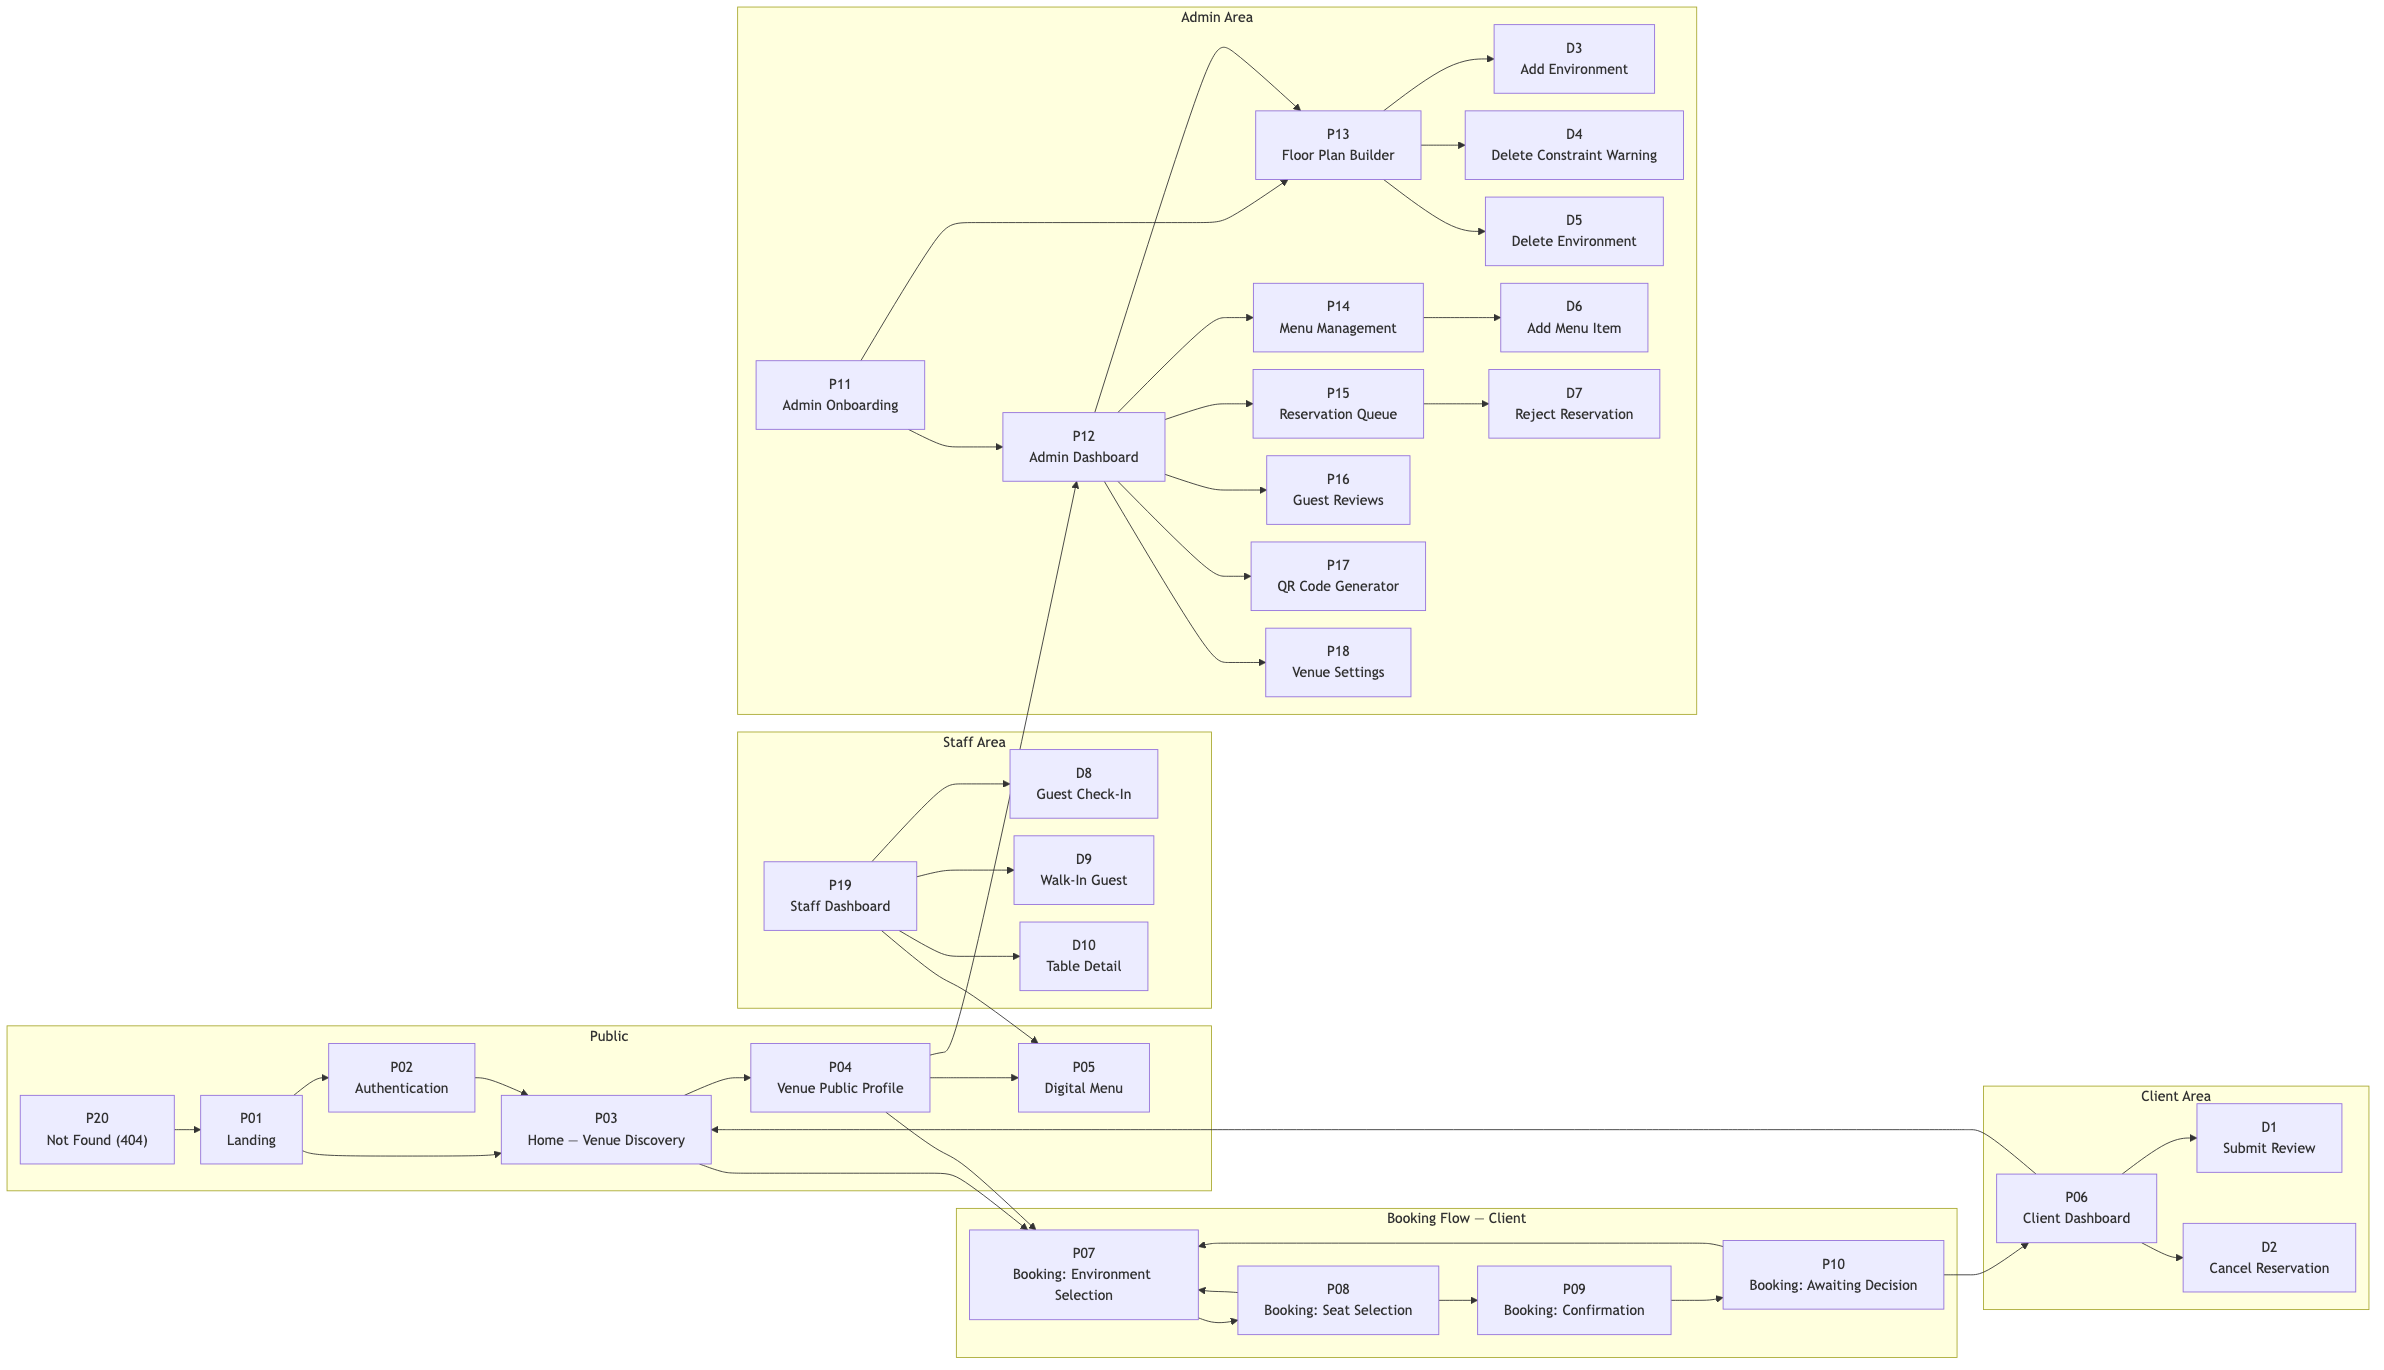
\includegraphics[width=0.97\linewidth]{nav.png}
  \caption{Spotly navigation diagram (landscape view for legibility)}
  \label{fig:nav}
\end{figure}
\end{landscape}

\section{Sketching}

The following pages present the wireframe views of the application, grouped
by functional area. Each wireframe is shown with a brief description of the
page's purpose.

% ── Public Area ──────────────────────────────────────────────────────────────
\subsection{Public Area}

\begin{figure}[H]
  \centering
  \begin{subfigure}[t]{0.47\linewidth}
    \centering
    \includegraphics[width=\linewidth]{P01_Landing.jpeg}
    \caption{P1 --- Landing page --- hero section and entry points for new and returning users.}
    \label{fig:wf:landing}
  \end{subfigure}
  \hfill
  \begin{subfigure}[t]{0.47\linewidth}
    \centering
    \includegraphics[width=\linewidth]{P02_Auth.jpeg}
    \caption{P2 --- Authentication page --- unified register and login form with tab switching.}
    \label{fig:wf:auth}
  \end{subfigure}
\end{figure}

\begin{figure}[H]
  \centering
  \begin{subfigure}[t]{0.47\linewidth}
    \centering
    \includegraphics[width=\linewidth]{P03_Home.jpeg}
    \caption{P3 --- Home page --- hero banner, discovery toggle (Search / Describe), venue grid.}
    \label{fig:wf:home}
  \end{subfigure}
  \hfill
  \begin{subfigure}[t]{0.47\linewidth}
    \centering
    \includegraphics[width=\linewidth]{P04_VenuePublicProfile.jpeg}
    \caption{P4 --- Venue public profile --- photo slideshow, identity details, reviews.}
    \label{fig:wf:profile}
  \end{subfigure}
\end{figure}

\begin{figure}[H]
  \centering
  \includegraphics[width=0.47\linewidth]{P05_DigitalMenu.jpeg}
  \caption{P5 --- Digital menu --- QR-routed, category tabs, environment-scoped items.}
  \label{fig:wf:menu}
\end{figure}

% ── Booking Flow ─────────────────────────────────────────────────────────────
\subsection{Booking Flow}

\begin{figure}[H]
  \centering
  \begin{subfigure}[t]{0.47\linewidth}
    \centering
    \includegraphics[width=\linewidth]{P07_BookingEnvironment.jpeg}
    \caption{P7 --- Step 1 --- environment selection: cards for each seating area.}
    \label{fig:wf:env}
  \end{subfigure}
  \hfill
  \begin{subfigure}[t]{0.47\linewidth}
    \centering
    \includegraphics[width=\linewidth]{P08_BookingSeats.jpeg}
    \caption{P8 --- Step 2 --- seat selection: visual floor plan with live table availability.}
    \label{fig:wf:seats}
  \end{subfigure}
\end{figure}

\begin{figure}[H]
  \centering
  \begin{subfigure}[t]{0.47\linewidth}
    \centering
    \includegraphics[width=\linewidth]{P09_BookingConfirm.jpg}
    \caption{P9 --- Step 3 --- confirmation form: guest details and submit button.}
    \label{fig:wf:confirm}
  \end{subfigure}
  \hfill
  \begin{subfigure}[t]{0.47\linewidth}
    \centering
    \includegraphics[width=\linewidth]{P10_BookingAwaiting.jpg}
    \caption{P10 --- Awaiting screen --- animated status timeline with real-time updates.}
    \label{fig:wf:awaiting}
  \end{subfigure}
\end{figure}

% ── Client Area ──────────────────────────────────────────────────────────────
\subsection{Client Area}

\begin{figure}[H]
  \centering
  \begin{subfigure}[t]{0.47\linewidth}
    \centering
    \includegraphics[width=\linewidth]{P06_ClientDashboard.jpeg}
    \caption{P6 --- Client dashboard --- upcoming and past reservations.}
    \label{fig:wf:clientdash}
  \end{subfigure}
  \hfill
  \begin{subfigure}[t]{0.47\linewidth}
    \centering
    \includegraphics[width=\linewidth]{P06_D1_SubmitReview.jpeg}
    \caption{D1 --- Submit review dialog --- star rating and written comment.}
    \label{fig:wf:review}
  \end{subfigure}
\end{figure}

\begin{figure}[H]
  \centering
  \includegraphics[width=0.47\linewidth]{P06_D2_CancelReservation.jpeg}
  \caption{D2 --- Cancel reservation confirmation dialog.}
  \label{fig:wf:cancel}
\end{figure}

% ── Admin Area ───────────────────────────────────────────────────────────────
\subsection{Admin Area}

\begin{figure}[H]
  \centering
  \begin{subfigure}[t]{0.47\linewidth}
    \centering
    \includegraphics[width=\linewidth]{P11_AdminOnboarding.jpg}
    \caption{P11 --- Admin onboarding wizard --- venue identity and first environment.}
    \label{fig:wf:onboarding}
  \end{subfigure}
  \hfill
  \begin{subfigure}[t]{0.47\linewidth}
    \centering
    \includegraphics[width=\linewidth]{P12_AdminDashboard.jpg}
    \caption{P12 --- Admin dashboard --- KPIs, environment overview, AI insights card.}
    \label{fig:wf:admindash}
  \end{subfigure}
\end{figure}

\begin{figure}[H]
  \centering
  \begin{subfigure}[t]{0.47\linewidth}
    \centering
    \includegraphics[width=\linewidth]{P13_FloorPlanBuilder.jpg}
    \caption{P13 --- Floor plan builder --- canvas with draggable table elements.}
    \label{fig:wf:floorplan}
  \end{subfigure}
  \hfill
  \begin{subfigure}[t]{0.47\linewidth}
    \centering
    \includegraphics[width=\linewidth]{P13_D3_AddEnvironment.jpg}
    \caption{D3 --- Add environment dialog --- name, icon, and gradient picker.}
    \label{fig:wf:addenv}
  \end{subfigure}
\end{figure}

\begin{figure}[H]
  \centering
  \begin{subfigure}[t]{0.47\linewidth}
    \centering
    \includegraphics[width=\linewidth]{P13_D4_DeleteConstraint.jpg}
    \caption{D4 --- Delete constraint dialog --- warns when active reservations exist.}
    \label{fig:wf:deleteconstraint}
  \end{subfigure}
  \hfill
  \begin{subfigure}[t]{0.47\linewidth}
    \centering
    \includegraphics[width=\linewidth]{P13_D5_DeleteEnvironment.jpg}
    \caption{D5 --- Delete environment confirmation dialog.}
    \label{fig:wf:deleteenv}
  \end{subfigure}
\end{figure}

\begin{figure}[H]
  \centering
  \begin{subfigure}[t]{0.47\linewidth}
    \centering
    \includegraphics[width=\linewidth]{P14_MenuManagement.jpg}
    \caption{P14 --- Menu management --- item list with category filter and availability toggles.}
    \label{fig:wf:menu-mgmt}
  \end{subfigure}
  \hfill
  \begin{subfigure}[t]{0.47\linewidth}
    \centering
    \includegraphics[width=\linewidth]{P14_D6_AddMenuItem.jpg}
    \caption{D6 --- Add / edit menu item dialog --- name, price, allergens, scope.}
    \label{fig:wf:additem}
  \end{subfigure}
\end{figure}

\begin{figure}[H]
  \centering
  \begin{subfigure}[t]{0.47\linewidth}
    \centering
    \includegraphics[width=\linewidth]{P15_ReservationQueue.jpg}
    \caption{P15 --- Reservation queue --- filterable list with approve/reject actions.}
    \label{fig:wf:queue}
  \end{subfigure}
  \hfill
  \begin{subfigure}[t]{0.47\linewidth}
    \centering
    \includegraphics[width=\linewidth]{P15_D7_RejectReservation.jpeg}
    \caption{D7 --- Reject reservation confirmation dialog.}
    \label{fig:wf:reject}
  \end{subfigure}
\end{figure}

\begin{figure}[H]
  \centering
  \begin{subfigure}[t]{0.47\linewidth}
    \centering
    \includegraphics[width=\linewidth]{P16_GuestReviews.jpg}
    \caption{P16 --- Guest review management --- list with hide/restore controls.}
    \label{fig:wf:reviews-mgmt}
  \end{subfigure}
  \hfill
  \begin{subfigure}[t]{0.47\linewidth}
    \centering
    \includegraphics[width=\linewidth]{P17_QRCodeGenerator.jpeg}
    \caption{P17 --- QR code generator --- per-table codes with download option.}
    \label{fig:wf:qr}
  \end{subfigure}
\end{figure}

\begin{figure}[H]
  \centering
  \includegraphics[width=0.47\linewidth]{P18_VenueSettings.jpeg}
  \caption{P18 --- Venue settings --- identity editor with photo gallery management.}
  \label{fig:wf:settings}
\end{figure}

% ── Staff Area ───────────────────────────────────────────────────────────────
\subsection{Staff Area}

\begin{figure}[H]
  \centering
  \begin{subfigure}[t]{0.47\linewidth}
    \centering
    \includegraphics[width=\linewidth]{P19_StaffDashboard.jpg}
    \caption{P19 --- Staff operations dashboard --- live floor map with waiter call alerts.}
    \label{fig:wf:staff}
  \end{subfigure}
  \hfill
  \begin{subfigure}[t]{0.47\linewidth}
    \centering
    \includegraphics[width=\linewidth]{P19_D8_GuestCheckIn.jpg}
    \caption{D8 --- Guest check-in dialog --- arrival confirmation with name and details.}
    \label{fig:wf:checkin}
  \end{subfigure}
\end{figure}

\begin{figure}[H]
  \centering
  \begin{subfigure}[t]{0.47\linewidth}
    \centering
    \includegraphics[width=\linewidth]{P19_D9_WalkInGuest.jpg}
    \caption{D9 --- Walk-in guest dialog --- instant reservation for unbooked arrivals.}
    \label{fig:wf:walkin}
  \end{subfigure}
  \hfill
  \begin{subfigure}[t]{0.47\linewidth}
    \centering
    \includegraphics[width=\linewidth]{P19_D10_TableDetail.jpg}
    \caption{D10 --- Table detail dialog --- current reservation info and status actions.}
    \label{fig:wf:tabledetail}
  \end{subfigure}
\end{figure}

\begin{figure}[H]
  \centering
  \includegraphics[width=0.47\linewidth]{P20_NotFound.jpg}
  \caption{P20 --- 404 Not Found page.}
  \label{fig:wf:404}
\end{figure}

\section{UI Design System}

Immediately after the sketching session, the team established a shared UI
design system to ensure visual consistency across all pages before implementation
began. This step was essential given that four members would be building
different parts of the interface in parallel.

The design system is built on top of Vuetify~3's theming engine and is defined
in a single \texttt{theme.js} file that the Vite plugin loads at startup.
Its core elements are:

\begin{itemize}[leftmargin=1.5em, topsep=4pt, itemsep=4pt]
  \item \textbf{Colour palette.} Two primary tokens drive the entire
        visual identity: \texttt{\#D4AF37} (champagne gold) for interactive
        elements, highlights, and the brand mark; and \texttt{\#0A0E14}
        (midnight black) for backgrounds and surface layers.
        A mid-grey (\texttt{\#555555}) is reserved for secondary text and
        borders. These tokens are exposed as both Vuetify theme colours and
        SCSS custom properties (\texttt{--color-gold}, \texttt{--color-bg})
        so that any component can consume them without hardcoding hex values.

  \item \textbf{Typography.} The heading typeface is set to a condensed
        serif to reinforce the luxury positioning; body text uses a clean
        sans-serif for readability. Both are declared in the theme so that
        Vuetify's \texttt{v-card}, \texttt{v-dialog}, and heading components
        inherit them automatically.

  \item \textbf{Component overrides.} Global defaults are applied to the
        most-used Vuetify components: \texttt{v-btn} (rounded corners, gold
        fill for primary variant), \texttt{v-card} (dark surface, subtle
        gold border), \texttt{v-chip} (gold outline for active filters), and
        \texttt{v-text-field} (underlined dark variant). This means every
        team member's pages share the same control appearance without
        per-component style repetition.

  \item \textbf{Spacing and layout tokens.} Standard spacing steps
        (4 px, 8 px, 16 px, 24 px) are documented and used consistently
        across all layouts so that the visual rhythm is uniform regardless
        of who built each page.
\end{itemize}

Having this system in place before any page was written meant that pull
requests from different members could be merged without visual inconsistency
reviews: the theme enforced correctness automatically.

\section{Data Model Diagram}

The class diagram in Figure~\ref{fig:class} shows the data model entities
used by the application, their fields, and their relationships. The diagram
reflects the final state after both phases of development. Each entity
corresponds to a file in \texttt{src/datamodel/} that exports a class, a
reactive list backed by \texttt{localStorage}, and CRUD functions.

Note that \textbf{user roles are not stored as a field} on the
\texttt{User} entity. The Admin role is derived at runtime by matching
\texttt{User.email} against \texttt{Venue.adminEmail}; the Staff role is
derived from the presence of a \texttt{VenueStaff} record; and the Client
role applies to any authenticated user who is neither an admin nor staff.

\begin{figure}[H]
  \centering
  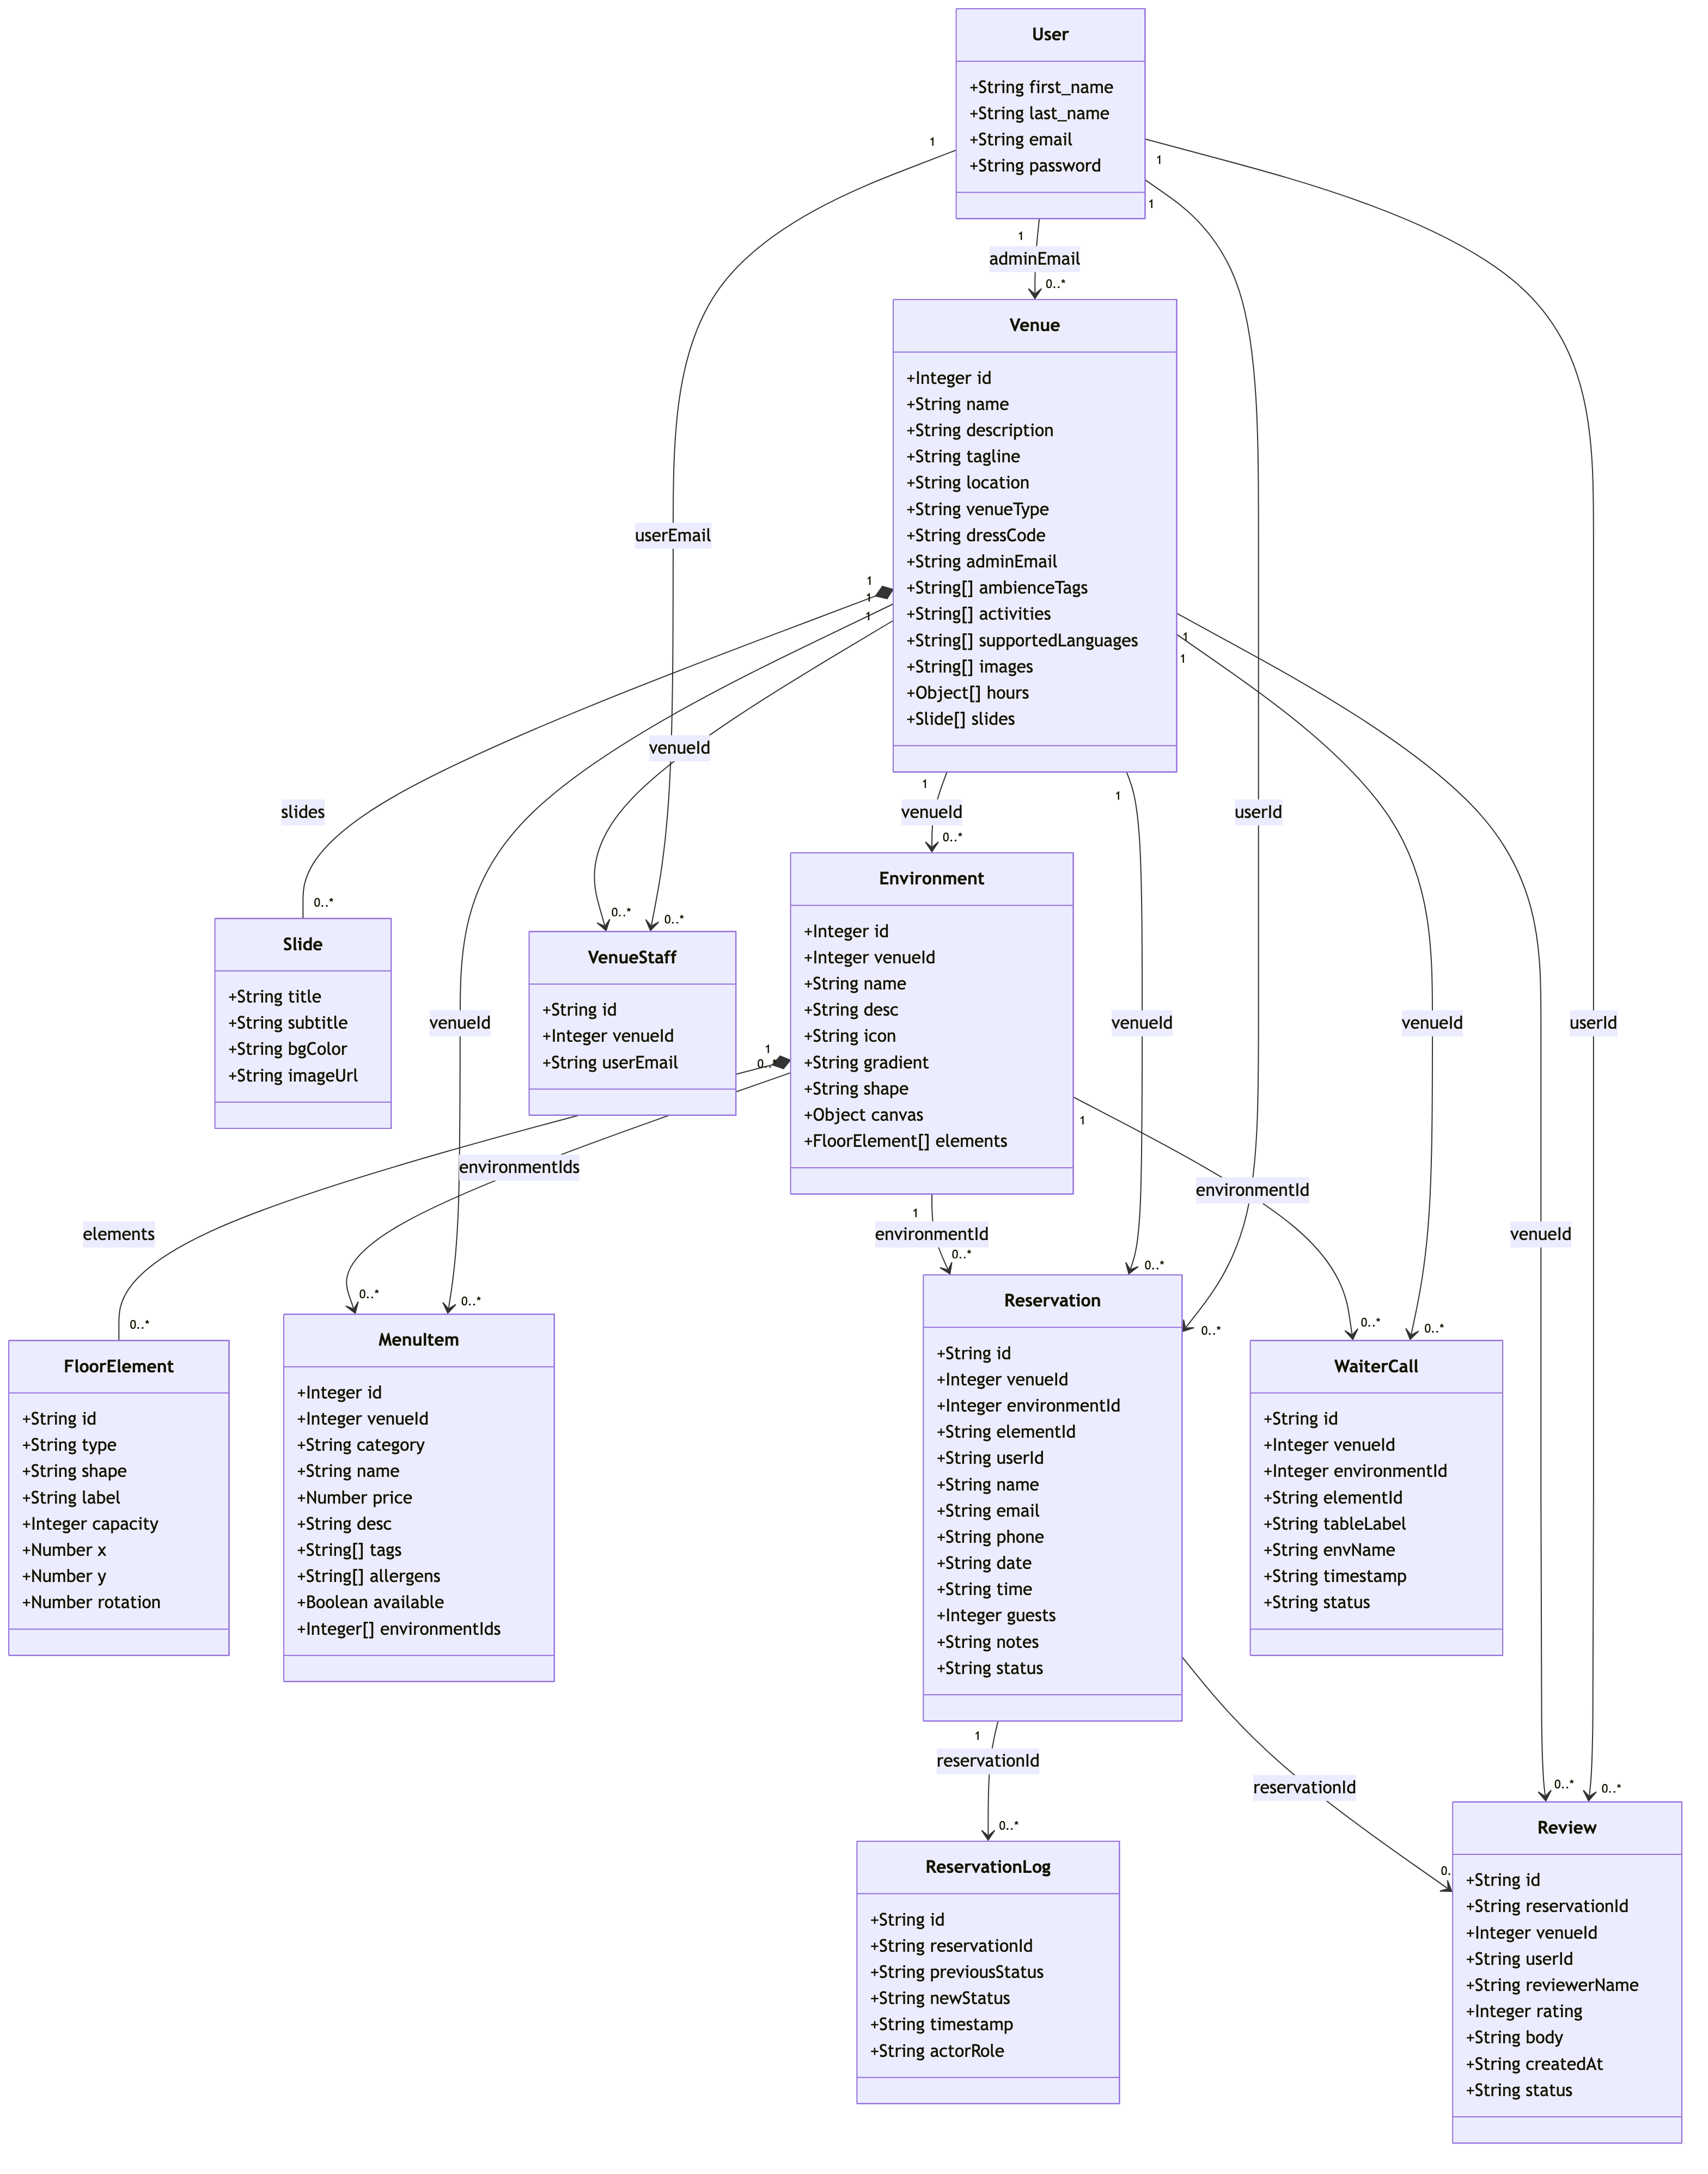
\includegraphics[width=0.98\linewidth]{class.png}
  \caption{Spotly data model class diagram}
  \label{fig:class}
\end{figure}

\textbf{Key entities and their primary fields:}

\begin{itemize}[leftmargin=1.5em, topsep=4pt, itemsep=3pt]
  \item \textbf{User} ---
    \texttt{first\_name, last\_name, email, password}.
    Storage key: \texttt{spotly\_users}.

  \item \textbf{Venue} ---
    Fields: id, name, description, tagline, location, venueType, adminEmail,
    ambienceTags, activities, dressCode, supportedLanguages, slides, hours.
    Storage key: \texttt{spotly\_venues}.

  \item \textbf{Environment} ---
    Fields: id, venueId, name, desc, icon, gradient, shape, canvas (width +
    height), elements.
    Element fields: id, type, shape, label, capacity, x, y, rotation.
    The element \texttt{status} is computed from reservations at render time
    and is never persisted.
    Storage key: \texttt{spotly\_environments}.

  \item \textbf{MenuItem} ---
    Fields: id, venueId, category, name, price, desc, tags, allergens,
    available, environmentIds.
    An empty \texttt{environmentIds} array means the item is venue-wide.
    Storage key: \texttt{spotly\_menu\_items}.

  \item \textbf{Reservation} ---
    Fields: id, venueId, environmentId, elementId, userId, name, email,
    phone, date, time, guests, notes, status.
    Statuses: REQUESTED, APPROVED, REJECTED, CANCELLED,
    CHECKED\_IN, COMPLETED, NO\_SHOW.
    Storage key: \texttt{spotly\_reservations}.

  \item \textbf{Review} ---
    Fields: id, reservationId, venueId, userId, reviewerName, rating,
    body, createdAt, status.
    Review statuses: VISIBLE, HIDDEN.
    Storage key: \texttt{spotly\_reviews}.

  \item \textbf{VenueStaff} ---
    Fields: id, venueId, userEmail.
    Storage key: \texttt{spotly\_venue\_staff}.

  \item \textbf{WaiterCall} ---
    Fields: id, venueId, environmentId, elementId, tableLabel, envName,
    timestamp, status.
    Call statuses: pending, acknowledged.
    Storage key: \texttt{spotly\_waiter\_calls}.
\end{itemize}

\section{Conclusion}

The three design artefacts --- navigation diagram, wireframe sketches, and
class diagram --- gave the team a shared understanding of the application's
structure before a single line of code was written. The class diagram in
particular proved invaluable: having stable entity definitions from the start
meant that every page could be wired to the data layer with confidence.
The diagrams were updated after Phase~2 to reflect the AI-driven flows.


% ═══════════════════════════════════════════════════════════════════════════════
\chapter{Project Implementation}
% ═══════════════════════════════════════════════════════════════════════════════

\section{Introduction}

This chapter describes the implementation of the Spotly platform: the hardware
and software environments used, the technology stack and its rationale, the
advanced AI features in technical depth, and the user interface screens.

\section{Hardware Environment}

\begin{tabularx}{\linewidth}{>{\bfseries}L{3cm} L{3cm} L{3.5cm} L{1.3cm} L{2.5cm}}
  \toprule
  Member & Machine & CPU & RAM & OS \\
  \midrule
  Cyrine Krichen   & HP Laptop           & Intel Core i7        & 32 GB & Windows 10 \\
  Eya Sassi        & Lenovo IdeaPad~3    & Intel Core i3-1115G4 & 8 GB  & Windows 11 \\
  Lina Khemiri     & Lenovo ThinkPad     & Intel Core i7        & 8 GB  & Windows 10 \\
  Youssef Ben Jemaa & MacBook Pro (2020) & Apple M1             & 8 GB  & macOS Sequoia \\
  \bottomrule
\end{tabularx}

\section{Software Environment}

\begin{tabularx}{\linewidth}{>{\bfseries}lX}
  \toprule
  Tool & Description \\
  \midrule
  Operating Systems & macOS Sequoia~15, Windows~11, Windows~10 \\
  \addlinespace
  IDE & Visual Studio Code with Volar (Vue language support) and
        ESLint extensions \\
  \addlinespace
  Browsers & Google Chrome (primary development and testing) and
             Firefox (cross-browser validation) \\
  \addlinespace
  Version Control & Git with GitHub (private repository) \\
  \addlinespace
  Package Manager & npm \\
  \addlinespace
  Build Tool & Vite~5 \\
  \addlinespace
  Design & Hand-drawn sketches (wireframes) \\
  \bottomrule
\end{tabularx}

\section{Technological Choices}

The table below lists every technology used in the project, its role, and the
rationale for its selection.

\begin{longtable}{>{\bfseries}L{3.8cm} L{3.2cm} L{5.5cm}}
  \toprule
  Technology & Role & Rationale \\
  \midrule
  \endfirsthead
  \toprule
  Technology & Role & Rationale \\
  \midrule
  \endhead
  \bottomrule
  \endlastfoot

  HTML5 &
    Markup structure &
    Semantic elements (\texttt{<section>}, \texttt{<article>}, \texttt{<nav>})
    improve accessibility and search discoverability. \\
  \addlinespace

  CSS3 + SCSS &
    Styling, design tokens &
    CSS custom properties (\texttt{--color-gold}, \texttt{--font-heading})
    centralise the design system. SCSS is compiled by Vite. \\
  \addlinespace

  JavaScript (ES2022+) &
    Application logic &
    Modern syntax (optional chaining, nullish coalescing, top-level await)
    reduces boilerplate. \\
  \addlinespace

  Vue.js~3 &
    Reactive component framework &
    Composition API with \texttt{<script setup>} enables co-located
    component logic without mixins. Fine-grained reactivity avoids
    unnecessary re-renders. \\
  \addlinespace

  Vuetify~3 &
    Material UI component library &
    Provides a comprehensive, accessible component set (data tables,
    dialogs, navigation drawers) that was customised with the champagne
    gold (\texttt{\#D4AF37}) palette. Eliminated weeks of custom component
    development. \\
  \addlinespace

  Vite~5 &
    Dev server and bundler &
    Sub-second hot module replacement during development. Native ES module
    support means no CommonJS bridging. \\
  \addlinespace

  \texttt{unplugin-}\newline\texttt{vue-router} &
    File-based routing &
    Routes auto-generated from the \texttt{src/pages/} directory tree.
    Dynamic segments use bracket syntax (\texttt{[id].vue}). \\
  \addlinespace

  \texttt{unplugin-}\newline\texttt{vue-components} &
    Auto-import &
    Vuetify and local components under \texttt{src/components/} are
    imported automatically, eliminating hundreds of explicit import lines. \\
  \addlinespace

  Cloudinary &
    Image hosting &
    Venue slideshow photos uploaded via unsigned upload preset.
    Cloudinary's CDN ensures fast delivery without a backend. \\
  \addlinespace

  \texttt{localStorage} &
    Client-side persistence &
    Provides synchronous read/write access to key--value storage.
    The \texttt{storage} event enables cross-tab reactivity with no
    WebSocket or polling required. \\
  \addlinespace

  Groq API &
    LLM inference &
    Free-tier API with low latency (\textasciitilde{}300--700~ms per turn).
    Compatible with the OpenAI chat completions schema, enabling tool
    calling. Model used: \texttt{meta-llama/} \texttt{llama-4-scout-17b-16e-instruct}. \\
  \addlinespace

  ElevenLabs API &
    Neural text-to-speech &
    Used in the voice agent for the AI assistant's voice output.
    Model: \texttt{eleven\_turbo\_v2\_5}, default voice: Rachel
    (\texttt{21m00Tcm4TlvDq8ikWAM}).
    Falls back gracefully to browser SpeechSynthesis when the key
    is absent. \\
  \addlinespace

  Web Speech Recognition API &
    Browser-native STT &
    Captures the user's voice during the reservation call.
    \texttt{continuous: false} with auto-restart on silence gives natural
    turn-taking behaviour. Chrome and Edge only. \\

\end{longtable}

\section{Advanced Technologies}

Following the completion of the core platform, the team explored AI integration
to further enhance the user experience. All three AI features use the same
\texttt{useAI} composable (\texttt{src/composables/useAI.js}), which wraps the
Groq API through a single \texttt{\_post} function. Two methods are exposed:
\texttt{callAI} (single-turn, system + user message) and
\texttt{callAIWithHistory} (multi-turn with tool call support).

\subsection{AI Semantic Venue Discovery (F22)}

The semantic discovery feature allows users to describe their desired atmosphere
in natural language and receive a ranked list of matching venues.

\subsubsection{Flow}
\begin{enumerate}[leftmargin=2em, topsep=4pt, itemsep=2pt]
  \item The user switches the home page discovery toggle from
        \emph{Search} to \emph{Describe with AI}.
  \item The user types a free-text description (e.g.\ ``\textit{a dark,
        intimate evening for a first date, ideally with live music}'').
  \item On clicking \emph{Find Venues}, the frontend constructs a venue
        payload: for each \texttt{Venue} in \texttt{VENUE\_LIST}, it
        serialises \texttt{id}, \texttt{name}, \texttt{description},
        \texttt{ambienceTags}, \texttt{activities}, and
        \texttt{dressCode} into a JSON array.
  \item The full venue list and the user's description are sent in a
        single-turn \texttt{callAI} request to the model.
  \item The model returns a JSON object with two keys:
        \texttt{summary} (a 4--6 word phrase capturing intent) and
        \texttt{venues} (a ranked array of \texttt{\{venueId, reason\}}
        objects, where \texttt{reason} is a max-12-word sentence citing
        something specific from the venue data).
  \item The frontend resolves each \texttt{venueId} to its
        \texttt{Venue} object and renders the cards in ranked order with
        gold match-reason badges.
\end{enumerate}

\subsubsection{Implementation notes}
The prompt instructs the model to return \textbf{only} valid JSON and
forbids inventing features not present in the venue data. A lightweight
validation check (\texttt{!result?.venues || !Array.isArray(result.venues)})
catches malformed responses and falls back to an error toast. The
\texttt{maxTokens} parameter is capped at 512 to minimise latency.

\subsection{AI Reservation Insights (F23)}

The insights feature gives venue administrators on-demand analytical
observations about their booking patterns.

\subsubsection{Payload aggregation}

When the admin clicks \emph{Generate}, the \texttt{computeInsightPayload}
function aggregates the past 30 days of reservation data from
\texttt{RESERVATION\_LIST} into a structured object:

\begin{itemize}[leftmargin=1.5em, topsep=2pt, itemsep=2pt]
  \item \textbf{Total} reservations in the period.
  \item \textbf{Status breakdown} (\texttt{byStatus}): count per
        \texttt{REQUESTED}, \texttt{APPROVED}, \texttt{CANCELLED},
        \texttt{NO\_SHOW}, etc.
  \item \textbf{No-show rate} and \textbf{cancellation rate} as
        percentages.
  \item \textbf{Day-of-week distribution} (\texttt{byDayOfWeek}):
        reservation count per weekday.
  \item \textbf{Hour distribution} (\texttt{byHour}): reservation count
        per hour slot.
  \item \textbf{Peak hour} and \textbf{quietest day}.
  \item \textbf{Average guest count} across all reservations.
  \item \textbf{Walk-in ratio}: proportion of reservations with no
        \texttt{elementId} (created by the staff walk-in dialog).
  \item \textbf{Top occasions}: keywords extracted from reservation
        notes (birthday, anniversary, proposal, business, date night)
        that appear in at least two reservations.
\end{itemize}

The serialised JSON payload is sent as the user message; the system prompt
instructs the model to return an array of 3--5 insights, each with an
\texttt{mdi} icon name, a severity (\texttt{info} / \texttt{warning} /
\texttt{success}), and a max-20-word sentence citing at least one number.

\subsubsection{7-Day Outlook tab}

A second AI card tab generates a forward-looking brief using
\texttt{computePredictivePayload}, which adds upcoming-week booking counts,
expected guest totals, and historical no-show/cancellation rates to the
payload. The prompt asks for 2--4 operational observations (e.g.\ which
evening needs extra staffing).

\subsubsection{Follow-up Q\&A}

Beneath the insights list, the admin can ask a follow-up question in plain
text. A third \texttt{callAI} invocation uses a narrowly scoped system
prompt that restricts the model to answering questions about the reservation
data only, preventing off-topic responses.

\subsubsection{Persistence}

Generated insights are cached in \texttt{localStorage} under the key
\texttt{spotly\_ai\_insights\_\{venueId\}} so they survive page reloads
without re-generating.

\subsection{AI Voice Reservation Agent (F21)}

The voice reservation feature is the most technically sophisticated component
of the project. It is implemented as a \textbf{tool-calling agentic loop}
--- not a simple voice-to-text transcription. Understanding why it qualifies
as an agent requires understanding the agentic pattern and then the specific
way it was implemented here.

\subsubsection{What makes it an agent}

A chatbot responds to each user message with one reply and stops. An agent
runs an \textbf{agentic loop}: the LLM receives the conversation history,
decides whether to speak or call a tool; if it calls a tool, the frontend
executes the tool and injects the result back into the conversation as a
\texttt{tool} role message; the model is then called again; and this
continues until the model produces a plain speech response. The loop is:

\[
\text{LLM} \;\xrightarrow{\text{tool call}}\; \text{frontend executor}
\;\xrightarrow{\text{tool result}}\; \text{LLM} \;\to\; \cdots
\;\xrightarrow{\text{speech response}}\; \text{user}
\]

In the Spotly voice agent, this loop is implemented as a \texttt{while(true)}
block inside the \texttt{sendTurn} function in
\texttt{VoiceCallModal.vue}. The loop breaks only when the model returns a
response with no \texttt{tool\_calls} (a plain speech turn). Tool call
chains can span multiple iterations within a single user utterance.

\subsubsection{The four tools}

\begin{description}[leftmargin=2em, topsep=4pt, itemsep=6pt,
                    font=\bfseries\ttfamily]
  \item[check\_availability]
    Given a \texttt{date} (ISO YYYY-MM-DD) and \texttt{guests} count, this
    tool queries \texttt{RESERVATION\_LIST} directly in \texttt{localStorage}.
    It filters each environment's table elements to those with sufficient
    capacity (\texttt{capacity >= guests}) and then checks every 30-minute
    time slot within the venue's configured opening hours for that environment
    to see if at least one eligible table is free. The response includes, for
    each environment: available slots and, when no slots exist, an
    \texttt{unavailableReason} field --- either \texttt{fully\_booked} or
    \texttt{no\_table\_large\_enough} --- so the model can give an accurate
    explanation to the guest. The model is instructed to call this tool
    \emph{immediately} when the guest mentions any date.

  \item[request\_text\_input]
    This tool creates a hybrid voice+text interaction: it renders a phone
    number entry card as a slide-up overlay in the call UI and then
    \textbf{suspends the agentic loop} by returning a \texttt{Promise} that
    only resolves when the guest types their number (8~digits, Tunisian
    format XX~XXX~XXX) and taps \emph{Confirm}. The loop resumes with the
    typed phone number injected as the tool result. Phone numbers are
    collected by typing rather than voice because speech-to-text transcription
    of digit sequences is unreliable.

  \item[confirm\_reservation]
    After the guest confirms their booking summary verbally, this tool
    performs full client-side validation before persisting: it checks that
    the date is not in the past, that the time falls within the venue's
    configured opening hours for the selected environment, and that a table with sufficient
    capacity is still free at that exact slot (a real-time check against
    \texttt{RESERVATION\_LIST}). On success, it constructs a
    \texttt{Reservation} object, calls \texttt{addReservation}, stores
    the new reservation's id in \texttt{sessionStorage} for the awaiting
    screen, and returns \texttt{\{success: true\}}. On failure, it returns
    an \texttt{error} payload (e.g.\ \texttt{no\_availability}) that the
    model relays naturally to the guest, prompting them to choose
    differently.

  \item[end\_call]
    Signals the call lifecycle to the frontend. A \texttt{reason} field
    distinguishes two outcomes: \texttt{reservation\_complete} (triggers
    a 2-second ``Reservation confirmed'' display then a redirect to the
    awaiting screen) and \texttt{user\_cancelled} (triggers a 1.8-second
    ``Call ended'' display then modal close). The model is instructed
    to call this tool after a farewell when the guest cancels, or after
    \texttt{confirm\_reservation} succeeds.
\end{description}

\subsubsection{Non-traditional aspects of this tool use}

\begin{itemize}[leftmargin=1.5em, topsep=4pt, itemsep=4pt]
  \item \textbf{No backend.} All tool execution happens entirely in the
        browser, directly against the \texttt{localStorage} data model.
        There is no server-side tool dispatcher.

  \item \textbf{Async suspension via Promise.} The
        \texttt{request\_text\_input} tool does not return immediately. It
        stores a resolver in component state and suspends. The UI renders
        the phone entry card. Only when the user types their number and
        confirms does the resolver fire, returning the phone value to the
        awaiting \texttt{await executeTool()} call, resuming the loop.

  \item \textbf{Full conversation history.} The \texttt{messages} array
        accumulates every turn with its role: \texttt{system},
        \texttt{user}, \texttt{assistant}, and \texttt{tool}. The model
        sees its own previous tool calls and results. This is what enables
        multi-step reasoning (e.g.\ the model can recall that
        \texttt{check\_availability} returned ``no table large enough''
        for environment A and suggest environment~B automatically).

  \item \textbf{Tool-call chaining.} After a single user utterance, the
        model may call \texttt{check\_availability} and then immediately
        infer an environment (without asking the guest) if only one
        environment has available slots. This chain completes before the
        model speaks its first word.

  \item \textbf{\texttt{parallel\_tool\_calls: false}.} The Groq API flag
        is explicitly set to \texttt{false} to prevent parallel tool
        invocations, which trigger a \texttt{tool\_use\_failed} error on
        this model. Tool calls are always sequential.

  \item \textbf{Recovery on malformed tool arguments.} If the model
        generates invalid JSON for tool arguments, the loop catches the
        error and retries once with the same history before falling back
        to a spoken ``Sorry, could you repeat that?'' and restarting STT.
\end{itemize}

\subsubsection{Voice I/O}

\textbf{Text-to-speech (TTS):}
The model's speech responses are first sent to the ElevenLabs API
(\texttt{eleven\_turbo\_v2\_5} model, Rachel voice) via a browser
\texttt{fetch} call. The response is an audio blob played through an HTML
\texttt{<audio>} element. If the API call fails or the key is absent, the
code falls back to \texttt{window.speechSynthesis}, selecting the best
available English voice.

\textbf{Speech-to-text (STT):}
The Web Speech Recognition API (\texttt{webkitSpeechRecognition} in
Chrome) listens with \texttt{continuous: false} and
\texttt{interimResults: false}. On every \texttt{result} event, the
transcript is passed immediately to \texttt{sendTurn}. On \texttt{end}
(silence detected), the recognition restarts automatically if the call is
still active, giving a natural turn-taking cadence. A \texttt{no-speech}
error also triggers a restart. STT is only available in Chrome and Edge.

\textbf{Call states:}
The UI models the call lifecycle through eight states:
\texttt{idle}, \texttt{opening}, \texttt{listening}, \texttt{thinking},
\texttt{speaking}, \texttt{done}, \texttt{cancelled}, and \texttt{error}.
Each state drives distinct ring animations: gold pulsing rings during
speaking, silver breathing rings during listening, and a spinning amber
ring during model inference.

\subsubsection{Live transcript}

A scrollable transcript panel (\texttt{.live-feed}) shows every turn in
real time: AI turns in gold, user turns dimmed, and tool invocations as
italic amber lines with a spinning gear icon. This transparency makes the
agentic loop visible to the user and aids debugging.

\section{User Interfaces}

% NOTE: These screenshots are placeholders (wireframe PNGs).
% They will be replaced by real application screenshots in the final submission.

The following pages present all views of the Spotly application, grouped by
area. The screenshots show the visual design built on Vuetify~3 with the
champagne gold palette.

% ── Public Area ──────────────────────────────────────────────────────────────
\subsection{Public Area}

\begin{figure}[H]
  \centering
  \begin{subfigure}[t]{0.47\linewidth}
    \centering
    \includegraphics[width=\linewidth]{P01_Landing.png}
    \caption{P1 --- Landing page}
    \label{fig:ui:landing}
  \end{subfigure}
  \hfill
  \begin{subfigure}[t]{0.47\linewidth}
    \centering
    \includegraphics[width=\linewidth]{P02_Auth.png}
    \caption{P2 --- Authentication page}
    \label{fig:ui:auth}
  \end{subfigure}
\end{figure}

\begin{figure}[H]
  \centering
  \begin{subfigure}[t]{0.47\linewidth}
    \centering
    \includegraphics[width=\linewidth]{P03_Home.png}
    \caption{P3 --- Home page (venue discovery)}
    \label{fig:ui:home}
  \end{subfigure}
  \hfill
  \begin{subfigure}[t]{0.47\linewidth}
    \centering
    \includegraphics[width=\linewidth]{P04_VenuePublicProfile.png}
    \caption{P4 --- Venue public profile}
    \label{fig:ui:profile}
  \end{subfigure}
\end{figure}

\begin{figure}[H]
  \centering
  \includegraphics[width=0.47\linewidth]{P05_DigitalMenu.png}
  \caption{P5 --- Digital menu (QR-accessed)}
  \label{fig:ui:digitalmenu}
\end{figure}

% ── Booking Flow ─────────────────────────────────────────────────────────────
\subsection{Booking Flow}

\begin{figure}[H]
  \centering
  \begin{subfigure}[t]{0.47\linewidth}
    \centering
    \includegraphics[width=\linewidth]{P07_BookingEnvironment.png}
    \caption{P7 --- Environment selection}
    \label{fig:ui:env}
  \end{subfigure}
  \hfill
  \begin{subfigure}[t]{0.47\linewidth}
    \centering
    \includegraphics[width=\linewidth]{P08_BookingSeats.png}
    \caption{P8 --- Seat and table selection}
    \label{fig:ui:seats}
  \end{subfigure}
\end{figure}

\begin{figure}[H]
  \centering
  \begin{subfigure}[t]{0.47\linewidth}
    \centering
    \includegraphics[width=\linewidth]{P09_BookingConfirm.png}
    \caption{P9 --- Reservation confirmation form}
    \label{fig:ui:confirm}
  \end{subfigure}
  \hfill
  \begin{subfigure}[t]{0.47\linewidth}
    \centering
    \includegraphics[width=\linewidth]{P10_BookingAwaiting.png}
    \caption{P10 --- Awaiting admin decision}
    \label{fig:ui:awaiting}
  \end{subfigure}
\end{figure}

% ── Client Area ──────────────────────────────────────────────────────────────
\subsection{Client Area}

\begin{figure}[H]
  \centering
  \begin{subfigure}[t]{0.47\linewidth}
    \centering
    \includegraphics[width=\linewidth]{P06_ClientDashboard.png}
    \caption{P6 --- Client dashboard}
    \label{fig:ui:clientdash}
  \end{subfigure}
  \hfill
  \begin{subfigure}[t]{0.47\linewidth}
    \centering
    \includegraphics[width=\linewidth]{P06_D1_SubmitReview.png}
    \caption{D1 --- Submit review dialog}
    \label{fig:ui:submitreview}
  \end{subfigure}
\end{figure}

\begin{figure}[H]
  \centering
  \includegraphics[width=0.47\linewidth]{P06_D2_CancelReservation.png}
  \caption{D2 --- Cancel reservation dialog}
  \label{fig:ui:cancelres}
\end{figure}

% ── Admin Area ───────────────────────────────────────────────────────────────
\subsection{Admin Area}

\begin{figure}[H]
  \centering
  \begin{subfigure}[t]{0.47\linewidth}
    \centering
    \includegraphics[width=\linewidth]{P11_AdminOnboarding.png}
    \caption{P11 --- Venue onboarding wizard}
    \label{fig:ui:onboarding}
  \end{subfigure}
  \hfill
  \begin{subfigure}[t]{0.47\linewidth}
    \centering
    \includegraphics[width=\linewidth]{P12_AdminDashboard.png}
    \caption{P12 --- Admin dashboard}
    \label{fig:ui:admindash}
  \end{subfigure}
\end{figure}

\begin{figure}[H]
  \centering
  \begin{subfigure}[t]{0.47\linewidth}
    \centering
    \includegraphics[width=\linewidth]{P13_FloorPlanBuilder.png}
    \caption{P13 --- Floor plan builder}
    \label{fig:ui:floorplan}
  \end{subfigure}
  \hfill
  \begin{subfigure}[t]{0.47\linewidth}
    \centering
    \includegraphics[width=\linewidth]{P13_D3_AddEnvironment.png}
    \caption{D3 --- Add environment dialog}
    \label{fig:ui:addenv}
  \end{subfigure}
\end{figure}

\begin{figure}[H]
  \centering
  \begin{subfigure}[t]{0.47\linewidth}
    \centering
    \includegraphics[width=\linewidth]{P13_D4_DeleteConstraint.png}
    \caption{D4 --- Delete constraint warning}
    \label{fig:ui:constraint}
  \end{subfigure}
  \hfill
  \begin{subfigure}[t]{0.47\linewidth}
    \centering
    \includegraphics[width=\linewidth]{P13_D5_DeleteEnvironment.png}
    \caption{D5 --- Delete environment confirmation}
    \label{fig:ui:deleteenv}
  \end{subfigure}
\end{figure}

\begin{figure}[H]
  \centering
  \begin{subfigure}[t]{0.47\linewidth}
    \centering
    \includegraphics[width=\linewidth]{P14_MenuManagement.png}
    \caption{P14 --- Menu management}
    \label{fig:ui:menumgmt}
  \end{subfigure}
  \hfill
  \begin{subfigure}[t]{0.47\linewidth}
    \centering
    \includegraphics[width=\linewidth]{P14_D6_AddMenuItem.png}
    \caption{D6 --- Add / edit menu item}
    \label{fig:ui:additem}
  \end{subfigure}
\end{figure}

\begin{figure}[H]
  \centering
  \begin{subfigure}[t]{0.47\linewidth}
    \centering
    \includegraphics[width=\linewidth]{P15_ReservationQueue.png}
    \caption{P15 --- Reservation queue management}
    \label{fig:ui:queue}
  \end{subfigure}
  \hfill
  \begin{subfigure}[t]{0.47\linewidth}
    \centering
    \includegraphics[width=\linewidth]{P15_D7_RejectReservation.png}
    \caption{D7 --- Reject reservation dialog}
    \label{fig:ui:rejectdialog}
  \end{subfigure}
\end{figure}

\begin{figure}[H]
  \centering
  \begin{subfigure}[t]{0.47\linewidth}
    \centering
    \includegraphics[width=\linewidth]{P16_GuestReviews.png}
    \caption{P16 --- Guest review management}
    \label{fig:ui:reviewmgmt}
  \end{subfigure}
  \hfill
  \begin{subfigure}[t]{0.47\linewidth}
    \centering
    \includegraphics[width=\linewidth]{P17_QRCodeGenerator.png}
    \caption{P17 --- QR code generator}
    \label{fig:ui:qr}
  \end{subfigure}
\end{figure}

\begin{figure}[H]
  \centering
  \includegraphics[width=0.47\linewidth]{P18_VenueSettings.png}
  \caption{P18 --- Venue identity and settings}
  \label{fig:ui:settings}
\end{figure}

% ── Staff Area ───────────────────────────────────────────────────────────────
\subsection{Staff Area}

\begin{figure}[H]
  \centering
  \begin{subfigure}[t]{0.47\linewidth}
    \centering
    \includegraphics[width=\linewidth]{P19_StaffDashboard.png}
    \caption{P19 --- Staff operations dashboard}
    \label{fig:ui:staff}
  \end{subfigure}
  \hfill
  \begin{subfigure}[t]{0.47\linewidth}
    \centering
    \includegraphics[width=\linewidth]{P19_D8_GuestCheckIn.png}
    \caption{D8 --- Guest check-in dialog}
    \label{fig:ui:checkin}
  \end{subfigure}
\end{figure}

\begin{figure}[H]
  \centering
  \begin{subfigure}[t]{0.47\linewidth}
    \centering
    \includegraphics[width=\linewidth]{P19_D9_WalkInGuest.png}
    \caption{D9 --- Walk-in guest dialog}
    \label{fig:ui:walkin}
  \end{subfigure}
  \hfill
  \begin{subfigure}[t]{0.47\linewidth}
    \centering
    \includegraphics[width=\linewidth]{P19_D10_TableDetail.png}
    \caption{D10 --- Table detail dialog}
    \label{fig:ui:tabledetail}
  \end{subfigure}
\end{figure}

\begin{figure}[H]
  \centering
  \includegraphics[width=0.47\linewidth]{P20_NotFound.png}
  \caption{P20 --- 404 Not Found page}
  \label{fig:ui:notfound}
\end{figure}

\section{Conclusion}

Chapter~4 documented the full implementation of Spotly. The technology
choices --- Vue.js~3, Vuetify~3, Vite, and \texttt{localStorage} --- formed
a coherent stack that allowed rapid development without a backend. The
\texttt{storage} event pattern, replicated across all eight data model files,
was the key to making cross-tab reactivity work seamlessly. The Advanced
Technologies section detailed the three AI features; the voice reservation
agent, in particular, demonstrates a genuinely agentic pattern --- tool calling,
async suspension, and real-time UI feedback --- in a frontend-only context.


% ═══════════════════════════════════════════════════════════════════════════════
\chapter*{General Conclusion}
\addcontentsline{toc}{chapter}{General Conclusion}
\markboth{General Conclusion}{}
% ═══════════════════════════════════════════════════════════════════════════════

Spotly started as an academic requirement and became something we are genuinely
proud of. Over the course of a single semester, the team went from a blank
repository to a feature-complete, visually polished venue discovery and booking
platform --- and then went further, building AI capabilities that none of us had
planned for at the outset.

\textbf{Goals reached.}
All 20 core features were implemented and are fully functional. The booking
flow (F5--F9) works end-to-end, including real-time cross-tab status updates
that required careful \texttt{storage} event wiring. The admin suite covers
every aspect of venue management. The staff dashboard handles the full shift
lifecycle. The three AI features add genuine value: semantic search makes
discovery feel conversational, the insights card turns raw data into
actionable observations, and the voice agent replaces a multi-step form with
a natural phone call.

\textbf{Challenges.}
The biggest technical challenge was designing the data layer. With no backend
and no state management library, we had to be disciplined: every entity
follows the same pattern (class, reactive list, CRUD functions, storage
watcher, cross-tab listener), and any deviation would have broken reactivity
across the app. We learned this discipline the hard way --- early pages that
mixed component-local arrays with the data layer produced hard-to-debug
inconsistencies. Once the pattern was established and respected, the
remaining pages went smoothly.

The voice reservation agent presented a different kind of challenge: making
an asynchronous agentic loop feel synchronous to the user. The
\texttt{request\_text\_input} tool's Promise-suspension mechanism --- pausing
the loop while the user types their phone number, then resuming it when they
confirm --- was the most creative piece of engineering in the project. It
took several iterations to get the state management right so that hanging up
mid-call would cleanly abort the loop at every \texttt{await} checkpoint.

\textbf{What we would do next.}
If the project continued, the most natural directions would be:

\begin{itemize}[leftmargin=1.5em, topsep=4pt, itemsep=3pt]
  \item \textbf{Backend migration}: replace \texttt{localStorage} with a
        real database and REST API, enabling multi-venue, multi-device access
        and proper authentication with hashed passwords.
  \item \textbf{AI table recommendation}: based on the guest's past
        preferences and party size, suggest the optimal table before they
        reach the seat selection step.
  \item \textbf{Predictive no-show detection}: use reservation history
        and contextual signals (day of week, time slot, party size) to flag
        reservations at high no-show risk so the admin can follow up
        proactively.
  \item \textbf{Multi-language support}: the platform already has a
        \texttt{supportedLanguages} field on venues; a natural next step
        would be a fully localised interface.
\end{itemize}

The AI features in particular felt like the beginning of something larger.
The voice agent --- a tool-calling LLM running entirely in the browser ---
demonstrates that sophisticated AI interactions do not require a dedicated
backend. That insight opens many possibilities for future work.

We leave this project with a solid command of modern frontend development,
a practical understanding of AI integration patterns, and a product we
would happily show to a real venue owner.


% ═══════════════════════════════════════════════════════════════════════════════
% APPENDIX
% ═══════════════════════════════════════════════════════════════════════════════
\appendix

\chapter{Use Case Scenarios}

This appendix presents the main use case scenarios of the Spotly platform.
Each scenario is assigned an identifier and is broken down into numbered steps
that indicate the involved user role and the relevant feature ID(s).
Scenarios S1--S8 cover the core Phase~1 features; scenarios S9--S11 cover
the AI-powered Phase~2 features.

% ═══════════════════════════════════════════════════════════════════════════
\section*{Phase 1 Scenarios}
% ═══════════════════════════════════════════════════════════════════════════

\subsection*{S1 --- Guest Explores the Platform Without an Account}
\begin{mdframed}[style=scenariobox]
\textbf{Actor:} Guest \quad
\textbf{Goal:} Discover available venues and browse the digital menu
without registering.
\end{mdframed}

\begin{longtable}{>{\bfseries}l L{6.2cm} l L{2.8cm}}
  \toprule
  Step & Description & Role & Features \\
  \midrule
  S1.1 & Guest opens the application and lands on the landing page. & Guest & F2 \\
  S1.2 & Guest clicks \emph{Explore Venues} and navigates to the home page
         without logging in. & Guest & F2 \\
  S1.3 & Guest browses the venue list and applies an activity filter. & Guest & F2 \\
  S1.4 & Guest clicks a venue card to open its public profile. & Guest & F3 \\
  S1.5 & Guest reads venue details, browses the photo slideshow, and views
         guest reviews. & Guest & F3 \\
  S1.6 & Guest scans a QR code at the venue and views the digital menu
         for their table. & Guest & F4 \\
  \bottomrule
\end{longtable}

\subsection*{S2 --- New Client Registers and Completes a Booking}
\begin{mdframed}[style=scenariobox]
\textbf{Actor:} Client \quad
\textbf{Goal:} Create an account and submit a table reservation at a
chosen venue.
\end{mdframed}

\begin{longtable}{>{\bfseries}l L{6.2cm} l L{2.8cm}}
  \toprule
  Step & Description & Role & Features \\
  \midrule
  S2.1 & Guest clicks \emph{Get Started} on the landing page and is redirected
         to the authentication page. & Guest & F1 \\
  S2.2 & Guest fills in first name, last name, email, and password, then clicks
         \emph{Register}. A session is created and the user is redirected to the
         home page as a Client. & Guest $\to$ Client & F1 \\
  S2.3 & Client searches for a venue by name using the search bar. & Client & F2 \\
  S2.4 & Client opens the venue profile page. & Client & F3 \\
  S2.5 & Client clicks \emph{Book a Table} to start the booking flow. & Client & F5 \\
  S2.6 & Client views available environments and selects one. & Client & F5 \\
  S2.7 & Client views the floor plan, picks an available table, and selects a
         date and time. & Client & F6 \\
  S2.8 & Client fills in guest details (name, email, phone, number of guests,
         optional notes) and clicks \emph{Submit Reservation}. & Client & F7 \\
  S2.9 & Client is redirected to the awaiting screen showing the animated status
         timeline. & Client & F8 \\
  \bottomrule
\end{longtable}

\subsection*{S3 --- Admin Processes a Reservation Request}
\begin{mdframed}[style=scenariobox]
\textbf{Actor:} Admin and Client \quad
\textbf{Goal:} Admin approves a pending reservation; client is notified in
real time.
\end{mdframed}

\begin{longtable}{>{\bfseries}l L{6.2cm} l L{2.8cm}}
  \toprule
  Step & Description & Role & Features \\
  \midrule
  S3.1 & Admin logs in and is redirected to the admin dashboard. & Admin & F1, F12 \\
  S3.2 & Admin notices a pending reservation count and navigates to the
         reservation queue. & Admin & F12, F15 \\
  S3.3 & Admin reads the reservation details: guest name, date, time,
         environment, table, and number of guests. & Admin & F15 \\
  S3.4 & Admin clicks \emph{Approve}; the reservation status changes to
         \texttt{APPROVED}. & Admin & F15 \\
  S3.5 & The client's awaiting screen detects the status change via the
         cross-tab storage event and the timeline advances without a page
         refresh. & Client & F8 \\
  S3.6 & Client is automatically redirected to the client dashboard. & Client & F8, F9 \\
  \bottomrule
\end{longtable}

\subsection*{S4 --- Client Manages Their Reservations and Leaves a Review}
\begin{mdframed}[style=scenariobox]
\textbf{Actor:} Client \quad
\textbf{Goal:} Cancel an upcoming reservation and submit a review for a past visit.
\end{mdframed}

\begin{longtable}{>{\bfseries}l L{6.2cm} l L{2.8cm}}
  \toprule
  Step & Description & Role & Features \\
  \midrule
  S4.1 & Client logs in and opens the client dashboard. & Client & F1, F9 \\
  S4.2 & Client views their upcoming reservations. & Client & F9 \\
  S4.3 & Client clicks \emph{Cancel} on a pending reservation; a confirmation
         dialog appears. & Client & F9 \\
  S4.4 & Client confirms cancellation; the reservation status updates to
         \texttt{CANCELLED}. & Client & F9 \\
  S4.5 & Client scrolls to the past visits section and finds a completed
         reservation without a review. & Client & F9, F10 \\
  S4.6 & Client clicks \emph{Write a Review}, selects a star rating, types a
         comment, and submits. & Client & F10 \\
  S4.7 & The review is published on the venue public profile. & Client & F10 \\
  \bottomrule
\end{longtable}

\subsection*{S5 --- Admin Onboards a New Venue}
\begin{mdframed}[style=scenariobox]
\textbf{Actor:} Admin \quad
\textbf{Goal:} Register as an admin and configure a new venue from scratch
to unlock the full admin panel.
\end{mdframed}

\begin{longtable}{>{\bfseries}l L{6.2cm} l L{2.8cm}}
  \toprule
  Step & Description & Role & Features \\
  \midrule
  S5.1 & New user registers via the authentication page and is redirected to
         the onboarding wizard (no venue exists yet). & Admin & F1, F11 \\
  S5.2 & Admin enters the venue name and basic identity details. & Admin & F11 \\
  S5.3 & Admin creates the first environment, completing the minimum onboarding
         requirement. & Admin & F11, F13 \\
  S5.4 & Admin is redirected to the floor plan builder. & Admin & F13 \\
  S5.5 & Admin adds table elements, sets their labels and capacities, and saves. & Admin & F13 \\
  S5.6 & Admin navigates to the admin dashboard, now fully accessible. & Admin & F12 \\
  \bottomrule
\end{longtable}

\subsection*{S6 --- Admin Configures the Venue for Operations}
\begin{mdframed}[style=scenariobox]
\textbf{Actor:} Admin \quad
\textbf{Goal:} Populate the menu, configure venue identity, and generate QR codes.
\end{mdframed}

\begin{longtable}{>{\bfseries}l L{6.2cm} l L{2.8cm}}
  \toprule
  Step & Description & Role & Features \\
  \midrule
  S6.1 & Admin opens the menu management page. & Admin & F14 \\
  S6.2 & Admin adds menu items across categories, filling in name, price,
         description, allergens, and tags. & Admin & F14 \\
  S6.3 & Admin assigns some items to specific environments only. & Admin & F14 \\
  S6.4 & Admin opens venue settings and updates the tagline, ambience tags,
         dress code, gallery photos, and opening hours. & Admin & F18 \\
  S6.5 & Admin opens the QR code generator and downloads codes for all tables. & Admin & F17 \\
  S6.6 & Admin navigates to guest review management and hides an inappropriate
         review. & Admin & F16 \\
  \bottomrule
\end{longtable}

\subsection*{S7 --- Staff Handles an Evening Shift}
\begin{mdframed}[style=scenariobox]
\textbf{Actor:} Staff \quad
\textbf{Goal:} Check in booked guests, handle a walk-in, and acknowledge a
waiter call.
\end{mdframed}

\begin{longtable}{>{\bfseries}l L{6.2cm} l L{2.8cm}}
  \toprule
  Step & Description & Role & Features \\
  \midrule
  S7.1 & Staff logs in and opens the staff operations dashboard. & Staff & F1, F19 \\
  S7.2 & Staff selects the current date and environment to load the live floor
         map. & Staff & F19 \\
  S7.3 & A guest with a confirmed reservation arrives; staff clicks their table
         and selects \emph{Check In}. Status changes to \texttt{CHECKED\_IN}. & Staff & F19 \\
  S7.4 & A second table's guest does not arrive; staff marks it as \emph{No-Show}.
         Status changes to \texttt{NO\_SHOW}. & Staff & F19 \\
  S7.5 & A walk-in party arrives; staff clicks \emph{Walk-In Guest}, fills in
         details, and a reservation is created instantly with status
         \texttt{CHECKED\_IN}. & Staff & F19 \\
  S7.6 & A table pulses gold indicating a waiter call; staff clicks
         \emph{Acknowledge} to dismiss it. & Staff & F20 \\
  S7.7 & At end of service, staff marks all occupied tables as \emph{Checked
         Out}. Statuses change to \texttt{COMPLETED}. & Staff & F19 \\
  \bottomrule
\end{longtable}

\subsection*{S8 --- Admin Rejects a Reservation}
\begin{mdframed}[style=scenariobox]
\textbf{Actor:} Admin and Client \quad
\textbf{Goal:} Admin rejects an unsuitable request; client is notified and
prompted to rebook.
\end{mdframed}

\begin{longtable}{>{\bfseries}l L{6.2cm} l L{2.8cm}}
  \toprule
  Step & Description & Role & Features \\
  \midrule
  S8.1 & Admin opens the reservation queue and locates a pending request that
         cannot be accommodated. & Admin & F15 \\
  S8.2 & Admin clicks \emph{Reject}; a confirmation dialog appears. & Admin & F15 \\
  S8.3 & Admin confirms; the reservation status changes to \texttt{REJECTED}. & Admin & F15 \\
  S8.4 & The client's awaiting screen detects the rejection via the storage event
         and displays a graceful decline card. & Client & F8 \\
  S8.5 & Client clicks \emph{Try Again}; the booking flow restarts from
         environment selection with the same venue pre-selected. & Client & F8, F5 \\
  \bottomrule
\end{longtable}

% ═══════════════════════════════════════════════════════════════════════════
\section*{Phase 2 Scenarios --- AI Features}
% ═══════════════════════════════════════════════════════════════════════════

\subsection*{S9 --- Client Books via Voice Call}
\begin{mdframed}[style=scenariobox]
\textbf{Actor:} Client \quad
\textbf{Goal:} Use the AI voice reservation agent to complete a full booking
through natural conversation.
\end{mdframed}

\begin{longtable}{>{\bfseries}l L{6.2cm} l L{2.8cm}}
  \toprule
  Step & Description & Role & Features \\
  \midrule
  S9.1 & Logged-in client sees the \emph{Voice Booking} option on the home page
         and taps the microphone button. & Client & F21 \\
  S9.2 & The full-screen voice call modal opens. The AI greets the client by
         name and asks how many guests will be joining. & Client & F21 \\
  S9.3 & Client says ``Two guests, this Friday evening.'' The agent calls
         \texttt{check\_availability} and reports available slots. & Client & F21 \\
  S9.4 & Client confirms an environment and time. The agent asks for the
         occasion and then calls \texttt{request\_text\_input}. & Client & F21 \\
  S9.5 & A phone number card slides up. Client types their number and taps
         \emph{Confirm}. The agent reads back a summary. & Client & F21 \\
  S9.6 & Client says ``Yes, confirm.'' The agent calls
         \texttt{confirm\_reservation}; the reservation is created. & Client & F21 \\
  S9.7 & The agent says goodbye and calls \texttt{end\_call}. The modal closes
         and the client is redirected to the awaiting screen. & Client & F21, F8 \\
  \bottomrule
\end{longtable}

\subsection*{S10 --- Client Discovers Venues via Natural Language Description}
\begin{mdframed}[style=scenariobox]
\textbf{Actor:} Client \quad
\textbf{Goal:} Use AI semantic discovery to find a venue matching a described
atmosphere.
\end{mdframed}

\begin{longtable}{>{\bfseries}l L{6.2cm} l L{2.8cm}}
  \toprule
  Step & Description & Role & Features \\
  \midrule
  S10.1 & Client opens the home page and switches the discovery toggle from
          \emph{Search} to \emph{Describe with AI}. & Client & F22 \\
  S10.2 & Client types: ``\textit{Somewhere dark and intimate for a first date,
          ideally with live jazz.}'' & Client & F22 \\
  S10.3 & Client clicks \emph{Find Venues}; venue cards are replaced with
          loading skeletons while the AI processes. & Client & F22 \\
  S10.4 & AI returns a ranked list. Cards reappear in ranked order, each with
          a gold badge showing the AI's match reason. & Client & F22, F2 \\
  S10.5 & Client selects the top match and opens its public profile. & Client & F3 \\
  S10.6 & Client starts the booking flow from the venue profile. & Client & F5 \\
  \bottomrule
\end{longtable}

\subsection*{S11 --- Admin Generates AI Insights About Reservation Patterns}
\begin{mdframed}[style=scenariobox]
\textbf{Actor:} Admin \quad
\textbf{Goal:} Use the AI insights card to understand booking trends and act
on them.
\end{mdframed}

\begin{longtable}{>{\bfseries}l L{6.2cm} l L{2.8cm}}
  \toprule
  Step & Description & Role & Features \\
  \midrule
  S11.1 & Admin opens the admin dashboard. & Admin & F12 \\
  S11.2 & Admin scrolls to the \emph{AI Insights} card and clicks
          \emph{Generate}. Skeleton rows appear while the AI processes. & Admin & F23 \\
  S11.3 & The system aggregates the last 30~days of reservation data (totals,
          no-show rate, peak hour, day-of-week distribution, average guests,
          top occasions) and sends it to the model. & Admin & F23 \\
  S11.4 & AI returns 3--5 observations, each with an icon and severity level.
          The card displays them as a list. & Admin & F23 \\
  S11.5 & Admin reads an insight flagging a high Friday no-show rate and
          decides to send reminder messages before future Friday reservations. & Admin & F23 \\
  \bottomrule
\end{longtable}

\end{document}
